\chapter{Teorema de Stokes}

\section{Lenguaje de las formas diferenciales}
\subsection{Casos específicos: 0, 1, y 2-formas}
\paragraph{0-formas}
\index{Formas!0}

Son funciones escalares definidas en un abierto de $\real^n$
\[\appl{f}{\Omega\subset\real^N}{\real}\]

Operaciones habituales:
\begin{itemize}
\item Suma: sí
\item Producto: sí
\item Composiciones: no (porque no cuadran las dimensiones)
\end{itemize}

\paragraph{1-formas}
\index{Formas!1}

Sea $\mathcal{C} = \{e_1,e_2,...,e_n\}$ la base canónica en $\real^N$.

Sea $L$ una aplicación lineal
\[\appl{L}{\real^N}{\real}\]

Que recordamos que cumplen:
\[ L(\gx+\gy) = L(\gx)+L(\gy); L(\lambda\gx) = \lambda L(\gx)\]

Definimos $\gy\in\real^N \leadsto \gy = \displaystyle\sum_1^n y_i e_i$, con lo que \[L(\gy) = \sum y_i L(e_i)\]

Entonces \[\left.\begin{array}{cc}
v_i = L(e_i)\\
y_i = P_i(\gy)
\end{array}\right\} \rightarrow L(\gy) = \sum_i v_iP_i(y)\]

Siendo $P_i$ las proyecciones, una base del espacio dual.

\textbf{Notación:}

$P_i \equiv dx_i$.

$dx_i[\gy] \equiv P_i(\gy) = y_i$

Entonces, dado un $\gv$ podemos construir 
\[L \equiv \sum_i^N v_idx_i\]

\[L[\gy] = \sum_i^N v_idx_i[\gy] = \sum_i^N v_iy_i\]

\begin{defn}[1-forma]
\[\omega(\gx)= \sum_1^N F_i(\gx) dx_i\]

\begin{itemize}
\item Se evalúa en $\gx\in\real$
\item Actúa sobre $\gy\in\real^N$ 
\end{itemize}

Es decir, \[\omega(\gx)[\gy] = \left(\sum F_i(\gx)dx_i\right)[\gy] = \sum F_i(\gx)dx_i[\gy] = \sum F_i(\gx)y_i\]
\end{defn}

Indicaremos con paréntesis el punto en el que estamos evaluando, y con corchetes el punto en el que estamso actuando.

\textbf{Operaciones:}
\begin{itemize}
\item Sumar: sí (lo razonable)
\item Multiplicar: por una función escalar sí está definida.
\end{itemize}


\paragraph{Ejemplo:}

Supongamos $f$ una función escalar (una 0-forma).

\[\grad f(\gx) = \left( \dpa{f}{x_i}(\gx)\right)\, i=1,...,N\]

Nos podemos construir una 1-forma desde el gradiente

\[\dpa{f}{x_i}(\gx)dx_i \]

A esta 1-forma en particular la llamaremos $df(\gx)$.

¿Utilidad? Ya la veremos, pero es una forma de escribir el producto escalar.
\[\pesc{\grad f(\gx),\gy} = df(\gx)[\gy]\]


\paragraph{2-formas}
\index{Formas!2}

Punto de partida: Aplicaciones \textbf{bilineales alternadas}

\[\appl{\Phi}{\real^N\x\real^N}{\real}\]

Que cumplen \begin{itemize}
\item $\Phi([\gu,\gv]) = - \Phi([\gv,\gu]) \implies \Phi(\gu,\gu)=0$
\item $ \Phi([\gu+\gv,\gw]) = \Phi ([\gu,\gw]) + \Phi([u,w])$
\item$\Phi([\lambda \gu,\gv]) = \lambda \Phi([\gu,\gv])$
\end{itemize}

Consecuencias:

\begin{itemize}
\item $\Phi(\gor{r}, \gor{s}+\gor{t}) = \Phi(\gor{r}+\gor{s}) + \Phi(\gor{r}+\gor{t})$
\item $\Phi(\gu,\mu\gv) = \mu\Phi(\gu,\gv)$
\end{itemize}


\paragraph{Ejemplo} en $\real^3$ para facilitar las cuentas.

\[\Phi(\gu,\gv) = \Phi(u_1e_1+u_2e_2+u_3e_3,v_1e_1+v_2e_2+v_3e_3)\]
Aplicando las propiedades anteriores obtenemos:

\begin{gather*}
\overbrace{u_1v_1\Phi(e_1,e_1)}^{\equiv 0} + u_1v_2\Phi(e_1,e_2) + u_1v_3+\Phi(e_1,e_3)+\\
u_2v_1+\Phi(e_2,e_1)+u_2v_2+\Phi(e_2,e_2)+u_2v_3+\Phi(e_2,e_3)+\\
u_3v_1\Phi(e_3,e_1)+u_3v_2+\Phi(e_3,e_2)+u_3v_3+\Phi(e_3,e_3) = \\
\underbrace{(u_1v_2-u_2v_1)}_{\left|\begin{matrix}
u_1&u_2\\v_1&v_2
\end{matrix}\right|}\overbrace{\Phi(e_1,e_2)}^{C_1}+(u_1v_3-u_3v_1)\Phi(e_1,e_3)+(u_2v_3-u_3v_2)\Phi(e_2,e_3)
\end{gather*}

Hemos demostrado que \[\Phi(\gu,\gv) = C_1B_{12}(\gu,\gv) + C_2B_{13}(\gu,\gv) + C_3B_{23}(\gu,\gv)\]

\subparagraph{Notación:} $B_{ij} = dx_i\y dx_j$

\[dx\y dx_j [\gu,\gv] = \det \begin{pmatrix}
u_i&u_j\\v_i&v_j
\end{pmatrix} = \det \begin{pmatrix}
dx_i[\gu]&dx_j[\gu]\\dx_[\gv]&dx_j[\gv]
\end{pmatrix}\]

\begin{defn}[2-forma]
\[\beta = \sum_{i,j=1}^N F_i(\gx) dx_i\y dx_j\]
\begin{itemize}
\item Se evalúan en puntos $x\in\real^N$
\item Actúan sobre pares de vectores $[\gu,\gv]\in\real^N\x\real^N$.
\end{itemize}

Es decir:

\[\beta(\gx)[\gu,\gv] = \sum F_{ij}(\gx) dx_i\y dx_j[\gu,\gv] = \sum F_{ij} \det \begin{pmatrix}
u_i&v_i\\u_j&v_j
\end{pmatrix}\]

\emph{Ojo} El cambio del orden (en el determiante)es aposta por la segunda propiedad de las 2 formas
\end{defn}


\subsection{Generalización: k-formas}
\index{k-forma}
\index{Formas!k}
Vamos a dar una definición general de una k-forma.

Elementos básicos:
\[\dfl{x_{i_1}}{x_{i_k}}[\gu^1,\gu^2,...,\gu^k] = \det\begin{pmatrix}
u_{i_1}^1 & ... & u_{i_k}^1\\
\vdots & \ddots & \vdots\\
u_{i_1}^k & ... & u_{i_k}^k
\end{pmatrix}\]

\begin{defn}[K-forma] Una k-forma es una expresión como la que sigue
\[
\sum_{i_1,...,i_k=1}^N F_{i_1,...,i_k}(\gx)\dfl{x_{i_1}}{x_{i_k}}
\]

Se evalúa en puntos $\gx\in\real^N$ y actúa sobre grupos de $K$ vectores.
\end{defn}

\begin{lemma} Si dos índices están repetidos, la diferencial vale 0:

\[ i_j = i_s \implies \df{x_{i_j},x_{i_s}} = 0 \]

\end{lemma}

Esto nos dice que en $\real^N$, teniendo $K$-formas (con $K<N$) tenemos $\comb{N}{K}$ combinaciones distintas.

\obs Si $K>N$ y $\omega$ es una k-forma, entonces $\omega \equiv 0$


\paragraph{Ejemplos:} En $\real^3$.

\begin{itemize}
\item 0-forma $\leadsto f(x,y,z) = 0$
\item 1-forma $\leadsto f_1(x,y,z)\df x + f_2(x,y,z)\df y + f_3(x,y,z)\df z$
\item 2-forma $\leadsto g_1(x,y,z)\df{y,z} + g_2(x,y,z)\df{z,x} + g_3(x,y,z)\df{x,y}$
\item 3-formas $\leadsto h(x,y,z)\df{x,y,z}$
\end{itemize}

\index{Orden!cíclico}
\emph{Ojo} Al cambio en la 2-forma, que es $dzdx$. Esto es para seguir el \textbf{orden cíclico} (por temas de la orientación). Esto es $x\to y \to z \to x$


\obs Las \textit{funciones escalares} las podemos interpretar como 0-formas y como 3-formas. Los \textit{campos vectoriales} los podemos interpretar como 1-formas y también como 2-formas.

\paragraph{Notación}
Para escribir un conjunto de subíndices $\{i_1,i_2,...,i_k\} \equiv I$

También acortaremos $\dfl{x_{i_1}}{x_{i_k}} \equiv dx_I$. 

La definición quedaría $\displaystyle \sum_I F_I(\gx)dx_I$

\subsection{Operaciones}
Siempre se puede multiplicar por 0-formas y sumar formas del mismo orden. Estas operaciones son triviales porque son operaciones internas.

Vamos a definir las operaciones externas:

\subsubsection{Producto exterior}

\begin{defn}[Producto\IS exterior]
Sean

\begin{gather*}
\omega = \sum_I F_I \df x_I\quad (\text{k-forma}\,\in\real^N) \\
\beta = \sum_J G_j \df x_J\quad (\text{s-forma}\,\in\real^N)
\end{gather*}

Se define el producto exterior de $ω$ y $β$ de la siguiente forma

\[\omega\y\beta = \sum_{I,J} F_IG_J \df{x_I,x_J} (\text{k+s-forma})\]
\end{defn}

\obs Si $K+S>N \implies \omega\y\beta=0$

Vamos a por un ejemplo de producto exterior en $ℝ^3$. Consideramos las dos siguientes formas diferenciales:

\begin{gather*}
\omega = f_1(x,y,z)\df x + f_2(x,y,z)\df y + f_3(x,y,z) \df z \\
\beta= g_1(x,y,z)\df x + g_2 (x,y,z) \df y + f_3 (x,y,z) \df z
\end{gather*}

y calculamos su producto exterior, $\omega\y\beta$

\begin{multline*}
\omega\y\beta  = f_1g_1\df{x,x} + f_1g_2\df{x,y} + f_1g_3\df{x,z} + f_2g_1\df{y,x} +\\  
+ f_2g_2\df{y,y}+ f_2g_3\df{y,z}  + f_3g_1\df{z,x}+f_3g_2\df{z,y}+f_3g_3\df{z,z}
\end{multline*}
Tachamos los que sean 0 ($\df{x,x} = 0$) y tenemos cuidado con el orden cíclico, y nos queda

\[ (f_2g_3-f_3g_2)\df{y,z} + (f_3g_1-f_1g_3)\df{z,x} + (f_1g_2 - f_2g_1) \df{x,y} \]

Partiendo de 2 campos vectoriales que eran 1-formas hemos llegado a una 2-forma. Además, si nos fijamos, hemos llegado a la definición de \textbf{producto vectorial} en $ℝ^3$: 

\[ \overrightarrow{F} \x \overrightarrow{G} = 
\left((f_2g_3-f_3g_2),(f_3g_1-f_1g_3),(f_1g_2 - f_2g_1)\right) \]

\subsubsection{Diferencial exterior}

El diferencial exterior trata de ampliar el concepto del diferencial (la matriz de derivadas parciales) más allá de las funciones, de tal forma que podamos aplicarlo a formas diferenciales.

\begin{defn}[Diferencial\IS exterior] Definimos la diferencial exterior de una k-forma como

\[\dif ω = \dif \left(\sum_I F_i(\gx)\df x_I\right) = \sum_I \underbrace{\df F_I}_{\text{1-forma}} \overbrace{\y}^{\text{Prod. ext}} \underbrace{\df x_I}_{\text{k-forma}} \]

donde 

\[ \dif f = \sum_i^N \dpa{f}{x_i} \df x_i \]

La diferencial exterior de una k-forma es una k+1-forma.
\end{defn}

Veamos algunos ejemplos, empezando en $ℝ^3$.

Partimos de un campo vectorial $G = (g_1,g_2,g_3)$ al que asociamos una 2-forma $ω$:

\[ \omega = g_1 \df{y,z} + g_2 \df{z,x} + g_3 \df{x,y} \]

Calculamos ahora la diferencial exterior, $\dif\omega$. Para calcularla, recordamos que $\df{x,x} = 0$ y que podemos cambiar el orden del producto exterior si respetamos el orden cíclico ($x,y,z$). 

\begin{align*}
\dif\omega 	&= 	\df{g_1,y,z} + \df{g_2,z,x} + \df{g_3,x,y} = \\
			&= 	\left(\dpa{g_1}{x} \df x + \dpa{g_1}{y} \df y + \dpa{g_1}{z}\df z \right)\y \df{y,z}\\ &\qquad  
			+	\left(\dpa{g_2}{x} \df x + \dpa{g_2}{y} \df y + \dpa{g_2}{z}\df z \right)\y \df{z,x}\\ &\qquad 
	 		+	\left(\dpa{g_3}{x} \df x + \dpa{g_3}{y} \df y + \dpa{g_3}{z}\df z \right)\y \df{x,y} = \\
			&= \dpa{g_1}{x}\df{x,y,z} + \dpa{g_2}{y}\df{y,z,x} + \dpa{g_3}{z}\df{z,x,y} = \\
			&= \left(\dpa{g_1}{x} + \dpa{g_2}{y} + \dpa{g_3}{z}\right)\df{x,y,z}
\end{align*}

Hemos llegado a una 3-forma que además es la forma diferencial asociada a la \textbf{divergencia} de $G$.

Pasamos a otro ejemplo, donde vamos a calcular la diferencial exterior de una 1-forma $ω=F_1\df x + F_2 \df y + F_3 \df z$. Recordamos que si invertimos el orden del producto exterior pagamos con un cambio de signo, esto es, $\df{x,z} = - \df{z,x}$.

\begin{align*}
\dif ω 	&= \dif\left(F_1\df x + F_2\df y+F_3\df z\right) =\\
		&= \df{F_1,x} + \df{F_2,y} + \df{F_3,z} = \\
		&= \left(\dpa{F_1}{x}\df x + \dpa{F_1}{x}\df y + \dpa{F_1}{x}\df z \right)\y \df x + 
		   \left(\dpa{F_2}{x}\df x + \dpa{F_2}{x}\df y + \dpa{F_2}{x}\df z \right)\y \df y + \\ & \qquad \qquad
		+  \left(\dpa{F_3}{x}\df x + \dpa{F_3}{x}\df y + \dpa{F_3}{x}\df z \right)\y \df z = \\
		&= \left(\dpa{F_3}{y} - \dpa{F_2}{z} \right)\df{y,z} + \left(\dpa{F_1}{z} - \dpa{F_3}{dx}\right)\df{z,x} + 
			\left(\dpa{F_2}{x} - \dpa{F_1}{y}\right) \df{x,y} 
\end{align*}

Nos ha quedado un campo de la forma:

\[\left(\left(\dpa{F_3}{y} - \dpa{F_2}{z} \right) ,\left(\dpa{F_1}{z} - \dpa{F_3}{x}\right),\left(\dpa{F_2}{x} - \dpa{F_1}{y}\right)\right)\]

que coincide con el \textbf{rotacional}.

\paragraph{Propiedades de la diferencial exterior}

\subparagraph{Diferencial de la suma} $\dif(\omega + \beta) = \dif\omega + \dif\beta$

\subparagraph{Diferencial del producto} Siendo $\omega = \sum_I F_I \dif x_I$ una k-forma, $f$ una 0-forma, tenemos que

\[ f\omega = \sum_I fF_I\dif x_I \]

y entonces
\[ \dif (f\omega) = \sum_I \df{(fF_I),x_I} \]

, donde \[ \dif (fF_I) = \sum_{j=1}^N \dpa{fF_I}{x_j} \df x_j = \sum_{j=1}^N\dpa{f}{x_j} F_I \df x_j + \sum_{j=1}^N\dpa{F_I}{x_j} f \df x_j = F_I \dif f + f \dif F_I \]

De esta forma, nos queda que 

\begin{align*}
\dif (fω)	&= \sum_I \left(F_I \dif f + f \dif F_I\right)\y \dif x_I = \\
			&= \sum_I F_I \df{f,x_I} + \sum_I f \df{F_I,x_I} = \\
			&= \sum_I \dif f \y F_I \dif x_I + f \dif ω = \\
			&= \dif f \y \left(\sum_I F_I \dif x_I\right) + f \dif ω = \\
			&= ω \df{f} + f \dif ω
\end{align*}

Hemos llegado a una expresión similar a la de la derivada de un producto de funciones

\[d(f\omega) = ω \df{f} + f \dif ω \]

\subparagraph{Diferencial del producto exterior} 

Sean dos k-formas diferenciales $ω$ y $β$:

\[ \omega =\sum f_i \df x_i ;\; \beta = \sum_j  g_j\df x_j \]

Calculamos el diferencial de su producto exterior:

\begin{align*}
\dif (\omega \y \beta) &= \dif\left(\sum_{i,j=1}^N f_ig_jdx_y\y dx_j\right) =\\
	&= \sum_{i,j=1}^N \df{(f_ig_j),x_i,x_j} = \\
	&= \sum_{i,j=1}^N \left(\sum_{k=1}^N \dpa{(f_ig_j)}{x_k} \dif x_k\right)\y \df{x_i,x_j} = \\
	&= \sum_{i,j,k=1}^N \left(\dpa{f_i}{x_k}g_j + f_i\dpa{g_j}{x_k}\right) \df{x_k,dx_i,dx_j} = \\
	&= \sum_{i,j,k=1}^N \dpa{f_i}{x_k}g_j \df{x_k,dx_i,dx_j}+ \sum_{i,j,k=1}^N f_i\dpa{g_j}{x_k}\df{x_k,dx_i,dx_j}
\end{align*}

Ahora tratamos de encontrar $ω$ y $β$ en ese engendro para volver a una expresión más agradable:

\begin{align*}
\dif (\omega \y \beta) &= \sum_{i,j,k=1}^N \dpa{f_i}{x_k}g_j \df{x_k,x_i,x_j}
	+ \sum_{i,j,k=1}^N f_i\dpa{g_j}{x_k}\df{x_k,dx_i,dx_j} \\
	&= \sum_{i,j,k=1}^N \dpa{f_i}{x_k}\df{x_k,x_i}\y(g_j\df x_j)
	+ \sum_{i,j,k=1}^N\dpa{g_j}{x_k}\df{x_k} \y f_i \df{x_i,dx_j} = \\
	&= \sum_{i} \left(\sum_k \dpa{f_i}{x_k}\df{x_k}\right) \y \dif x_i \y  \left(\sum_j g_j\dif x_j\right) \\ &\qquad
	+  \sum_{j} \left(\sum_k \dpa{g_j}{x_k}\df{x_k}\right) \y \left(\sum_i f_i\dif x_i\right) \y \dif x_j = \\
	&= \sum_i \df{f_i,x_i} \y β + \sum_j \df{g_j} \y ω \y \dif x_j = \\
	&= \left(\sum_i \df{f_i,x_i}\right) \y β - ω \y \left(\sum_j \df{g_j,x_j}\right) = \\
	&= \dif ω \y β - ω \y \dif β
\end{align*}

Entonces, si $\omega,\beta$ son 1-formas tenemos que $\dif(\omega \y \beta) = \dif\omega \y \beta - \omega \y\dif\beta$. Si por el contrario tuviésemos que $\omega$ es una k-forma y $\beta$ una s-forma, repitiendo las cuentas de nuevo llegaríamos a 

\[\dif \omega \y \beta + (-1)^k \omega \y \dif\beta\]

\subparagraph{Diferencial del diferencial} 

Sea $\omega$ k-forma con coeficientes $C^2$. Entonces, 

\[ \dif (\dif ω) = 0 \]

\paragraph{Propiedades del diferencial exterior} Resumiendo las propiedades del diferencial:
\index{Diferencial!propiedades}
\begin{itemize}
\item $\dif (ω + β) = \dif ω + \dif β$.
\item $\dif (fω) = ω \dif f + f \dif ω$.
\item $\dif (ω \y β) = \dif ω \y β + (-1)^k ω \y \dif β$ siendo $ω$ una k-forma.
\item $\dif(\dif ω) = 0$.
\end{itemize}
\subsubsection{Relación con operaciones en funciones vectoriales}

Partiendo de un campo en $\real^3$, podemos interpretarlo como una 1-forma o como una 2-forma. 

\begin{itemize}
\item La diferencial exterior de un campo interpretado como 1-forma es la 2-forma asociada a la \textbf{divergencia}.
\item La diferencial exterior de un campo interpretado como 2-forma es la 3-forma asociada al \textbf{rotacional}.
\item El producto exterior de 2 campos interpretados como 2-formas nos da el campo asociado al \textbf{producto vectorial}.
\item ¿Cómo tengo que interpretar los campos para conseguir un producto escalar?
\end{itemize} 


\subsubsection{Pull-back}
Queremos saber cómo llevar k-formas de $\real^N$ a $\real^M$. Partimos de la base de que existe una transformación $\appl{T}{ℝ^N}{ℝ^M}$ tal que $T(s)=x$, y buscamos otra aplicación $\appl{\pb}{\real^M}{\real^N}$.

En caso de 0-formas, el \emph{pull-back} es lo mismo que la composición. Es decir, dada una función $\appl{f}{ℝ^M}{ℝ}$, $\pb f = f \circ T$.

Basándonos en esta misma idea sobre las funciones escalares, vamos a tratar de hallar el pullback para las formas diferenciales. Supongamos que tenemos una k-forma $\omega$ en $\real^M$. Queremos construir $T^{\ast}$ en términos de $T$ y $\omega$. Partimos de  $\gor{s} \in \real^N$ (el punto donde se evalúa la k-forma), y $\gv_1,\gv_2,..,\gv_k$ los vectores en $\real^N$ sobre los que actúa $ω$. Entonces

\[
(T^{\ast}\omega)(\gor{s}) [\gv_1,\dotsc,\gv_k] = \omega(\underbrace{T(s)}_{\in\real^M}) [\underbrace{DT(s)\gv_j}_{\in\real^M}]
\]

Es decir, transformamos el punto en el que se evalúa $ω$, que pasa a ser $T(\gor{s})$ en lugar de $\gor{s}$, y los vectores sobre los que actúa también los "movemos" usando la matriz diferencial.

Vemos que 

\[\omega(T(s)) [DT(s)\gv]\equiv \sum f_i(T(s))\dif x_i[DT(s)\gv]\]

\[DT(s) = \begin{pmatrix}
\dpa{T_1}{s_1}(s) & ... & \dpa{T_1}{s_N}\\
\vdots & \ddots & \vdots \\
\dpa{T_M}{s_1} & \dots & \dpa{T_M}{s_N}
\end{pmatrix} \cdot \begin{pmatrix}
v_1\\
\downarrow\\
v_N
\end{pmatrix}\]

¿Que significa $\dif x_i[DT(s)\gv]$? Vamos a ver que pasa con el producto de una de las filas de la matriz.

\[\df{x_i} [DT(s)\gv] = \dpa{T_i}{s_1}v_1 + ... + \dpa{T_i}{s_N}v_n\]
Podemos darnos cuenta de que $v_1 = \dif s_1[\gv]$. Con esto tenemos:

\[\df{x_i} [DT(s)\gv] = \left(\dpa{T_i}{s_1}\dif s_1 + ... + \dpa{T_i}{s_N}\dif s_N \right)[\gv] = \dif T_i [\gv] \]

y por lo tanto

\[ (\pb ω)(\gor{s})[\sample[\gor{v}][k]] =  \omega(T(s)) [DT(s)\gv] = \sum f_i (T(s))  \dif T_i [\gv] \]

\paragraph{Ejemplos}

\subparagraph{Ej. 1)} Sea  $f(x)\dif x_i$ una 1-forma de la que queremos calcular el \emph{pull-back}

\[T^{\ast}(f\dif x_i)(s)[v] = f(T(s)) \dif x_1[DT(s)\gv]\]
Supongamos $f\equiv 1$
\[T^{\ast}(fdx_i)(s)[v] = \dif x_1[DT(s)\gv] = \dif T_i[\gv]\]
\textbf{Conclusión: } $T^{\ast}\dif x_i = \dif T_i$.

\subparagraph{Ej. 2)} Sea $\omega = \sum_i f_i \dif x_i$ una 1-forma de la que queremos calcular el \emph{pull-back}

\[ 
 (T^{\ast} \omega )(s)[\gv]= \sum_i f_i(T(s))\dif x_i [DT(s)\gv] = \sum_i f_i(T(s)) \dif T_i [\gv ] = T^{\ast} (\sum_i f_i \dif x_i ) = \sum_i f_i \circ T \dif T_i
\]

\textbf{Conclusión: } $T^{\ast} (\sum_i f_i\dif x_i) = \sum_i (f_i \circ T) \dif dT_i$

\subparagraph{Ej. 3: Pullback del producto exterior} ¿Cómo se comporta con el producto exterior? Vamos a trabajar con $f\equiv 1$.

\begin{gather*}
T^{\ast}(\df{x_i,x_j} [\gu,\gv] = \df{x_i,x_j} \left[DT(s)[\gu], DT(s)[\gv]\right] = \\
= \left|\begin{matrix}
	\dif x_i[DT(s)\gu] & \dif x_j[DT(s)\gu] \\
	\dif x_i[DT(s)\gv] & \dif x_j[DT(s)\gv] 
	\end{matrix}\right| 
= \left| \begin{matrix}
	\dif T_i[\gu] & \dif T_j[\gu]\\
	\dif T_i[\gv] & \dif T_j[\gv]
\end{matrix}\right| 
\stackrel{(1)}{=} \df{T_i,T_j} [\gu,\gv]
\end{gather*}
(1): Por las propiedades del producto exterior de 1-formas.

\textbf{Conclusión: } $T^{\ast} (dx_i \y dx_j) = dT_i \y dT_j$.

\subparagraph{Ej. 4)} ¿Qué pasa cuando tenemos el producto de 2-formas generadas?

\[\omega = \sum f_idx_i\,;\,\beta=\sum g_jdx_j\]
Vamos con el producto exterior.

\begin{gather*}
T^{\ast} (\omega \y \beta) (s) [\gu,\gv] = \sum_{i,j} f_i(T(s))g_j(T(s)) \underbrace{\df{x_i,x_j} [DT(s)\gu, DT(s),\gv]}_{\text{Calculado justo arriba}}\\
= \sum_{i,j} (f_i\circ T) = \dotsb \\
= \left(\sum (f_i\circ T)\dif T_i\right)\y\left(\sum(g_j \circ T) \dif T_j\right) = T^{\ast}\omega \y T^{\ast}\beta
\end{gather*}

\textbf{Conclusión: } $T^{\ast}(\omega \y \beta) = T^{\ast}\omega \y T^{\ast}\beta$. 

Esto es válido para multiíndices $I$, es decir, para $\omega$ k-forma y $\beta$ s-forma.


\paragraph{Pull-back y diferencial exterior}
Una vez visto cómo se comporta el \emph{pull-back} respecto del producto exterior vamos a ver como se comporta con respecto de la diferencial exterior.

\begin{gather*}
\dif (T^{\ast} \omega) = \dif \left(\sum_i f_i(T(s)) \dif x_i [DT(s)\gv]\right) = \dif\left(\sum (f_i \circ T)(s) \dif T_i[\gv]\right)\\
= \sum_i \dif(f_i\circ T)\y dT_i
\end{gather*}

Vamos a ver qué significa $\dif(f_i\circ T)$:

\begin{gather*}
\dif (f_i\circ T) =  \sum_k \dpa{f_i\circ T}{s_k} \dif s_k \\
\dpa{f_i\circ T}{s_k} = \sum_j \dpa{f_i}{x_j}(T(s))\cdot \dpa{x_j}{s_k}
\end{gather*}
Donde $x_j = T_j(s)$. Juntando todo tenemos: 

\[ 
\dif (T^{\ast} \omega) = \sum_{i,j,k} \dpa{f_i}{x_j}(T(s)) \dpa{T_j(s)}{s_k} \df{s_k,T_i} = \sum_{i,j} \dpa{f_i}{s_j}(T(s)) \df{T_j,T_i} = T^{\ast}(d(\sum f_i \dif x_i))
\]
 
 \textbf{Conclusión: } $\dif (T^{\ast}\omega) = T^{\ast}(\dif \omega)$
 
 
 \paragraph{Ejemplo concreto: Cambio a coordenadas polares} El cambio a coordenadas polares $(\rho,\theta)$ se define por la siguiente transformación:
  
 \[T(\rho,\theta) =\left( T_1(\rho,\theta),T_2(\rho,\theta)\right) = (\rho \cos\theta,\rho \sen\theta)\]
 
 Vamos a calcular los pull-backs:
 
 \begin{gather*}
 T^{\ast}(\dif x) = \dif T_1 = \dpa{T_1}{ρ}\dif ρ + \dpa{T_1}{θ}\dif θ = \cos θ \dif ρ - ρ \sen θ \dif θ \\
 T^{\ast}(\dif y) = \dif T_2 = \dpa{T_2}{ρ}\dif ρ + \dpa{T_2}{θ}\dif θ = \sen θ \dif ρ + ρ \cos θ \dif θ
 \end{gather*}
 
 Juntando ahora lo que tenemos:
 
\begin{align*}
\pb(\df{x,y}) &= (\pb \dif x) \y (\pb \dif y) = \\
	&= (\cos θ \dif ρ - ρ \sen θ \dif θ) \y (\sen θ \dif ρ + ρ \cos θ \dif θ) = \\
	&= ρ \cos^2 θ \df{ρ,θ} - ρ \sen^2 θ \df{θ,ρ} = \\
	&= \left(ρ \cos^2 θ + ρ \sen^2 θ\right) \df{ρ,θ} = \\
	&= ρ \df{ρ,θ}
\end{align*}

\paragraph{Propiedades fundamentales de la operación}
\index{Pullback!propiedades}
\begin{enumerate}
\item $T^\ast f = f\circ T$, siendo $f$ una 0-forma.
\item $T^\ast(dω) = d(T^\ast ω)$. En particular $T^\ast (dx_I) = dT_I$.
\item $T^\ast(ω\y β)=(T^\ast ω) \y (T^\ast β)$.
\item $T^\ast(fω) = (f\circ T)(T^\ast ω) = (T^\ast f)(T^\ast ω)$
\item $T^\ast(ω+β)=T^\ast+T^\ast β$.
\item $(T\circ S)^\ast ω = S^\ast(T^\ast ω)$.
\end{enumerate}

\begin{example} Tenemos una aplicación $φ(s,t) = (φ_1(s,t), φ_2(s,t))$. Calculamos su pullback y entonces

\[ φ^\ast(\dif x) = \dif φ_1 = \dpa{φ_1}{s}\dif s + \dpa{φ_1}{t}\dif t \]

y de la misma forma
\[ φ^\ast(\dif y) = \dif φ_2 = \dpa{φ_2}{s}\dif s + \dpa{φ_2}{t}\dif t \]

\begin{gather*}
 φ^\ast(dx\y dy) = dφ_1\y dφ_2 =\left( \dpa{φ_1}{s}ds + \dpa{φ_1}{t}dt \right) \y\left( \dpa{φ_2}{s}ds + \dpa{φ_2}{t}dt \right) = \\
 0 + \dpa{φ_1}{s}\dpa{φ_2}{t}ds\y dt + \dpa{φ_1}{t}\dpa{φ_2}{s} dt\y ds + 0
 \end{gather*}
 
 Los diferenciales están cambiados de orden así que seguimos pagando con un cambio de signo:
 
 \[ \left(\dpa{φ_1}{s}\dpa{φ_2}{t} - \dpa{φ_1}{t}\dpa{φ_2}{s}\right)ds\y dt= \left|\begin{matrix}
 \dpa{φ_1}{s} & \dpa{φ_1}{t} \\
 \dpa{φ_2}{s} & \dpa{φ_2}{t} 
 \end{matrix}\right| =  \det \left(\dpa{φ}{s,t}\right) ds\y dt \]
 \end{example}
 
 \begin{example}
 Tenemos $β$, la 2-forma asociada a un campo $\vf=(F_1, F_2, F_3)$:
 
 \[ β = F_1\df{y,z} + F_2\df{z,x} + F_3 \df{x,y} \]
 
 Queremos calcular su pullback mediante una aplicación $\appl{Φ}{ℝ^2}{ℝ^3}$. Entonces
 
 \[ Φ^\ast β = g(s,t) \df{s,t} \]
 
 ¿Quién es $g$? Calculamos el pullback:
 
 \[ φ^\ast β = F_1\circ Φ\df{Φ_2,Φ_3} + F_2\circ Φ\df{Φ_3,Φ_2} + F_3\circ Φ\df{Φ_1,Φ_2} \]
 
 Calculamos los distintos diferenciales, que no pienso copiarlos porque no los ha puesto él en la pizarra, y los pinchamos en el morcillo ese. Y operamos. Y yo no voy a operar. Al final sale todo y queda lo siguiente
 
 \[ =\pesc{\vf\circ Φ, \left(\dpa{Φ_1}{s}, \dpa{Φ_2}{s}, \dpa{Φ_3}{s}\right) × \left(\dpa{Φ_1}{t}, \dpa{Φ_2}{t}, \dpa{Φ_3}{t}\right)} \df{s,t} \]
 
 Sin embargo, el producto vectorial de esos dos vectores parece el producto vectorial de $T_s × T_x$, el factor que teníamos que poner para integrar un campo en una superficie. Poderosa magia hombre blanco.
 \end{example}
 
 \begin{example} Tenemos una 1-forma asociada a $\vf$:

 \[ ω = \sum_i F_i\dif x_i \]
 
 y una aplicación (curva) $\appl{σ}{ℝ}{ℝ^n}$. Entonces $σ^\ast ω$ es de la forma $g(t)\dif t$. 
 
 Entonces
 
 \begin{gather*} (σ^\ast ω)(t)[λ] = \sum_i F_i(σ(t)) \dif x_i[Dσ(t)λ] = \sum_i F_i(σ(t)) \dif x_i[σ_1'(t)λ, \dotsc, σ_N'(t)λ = \\
 = \sum_i F_i(σ(t)) σ_i'(t) \dif t[λ] = \\
 = \pesc{\vf \circ σ, σ'} \dif t [λ]
 \end{gather*}
 
 Que, oh, sorpresa de nuevo, es lo que aparece cuando integrábamos un campo sobre una curva. 
 \end{example}
 
 Al final, querremos integrar k-formas en $ℝ^N$ sobre variedades de dimensión $k$. 
 
\section{Integración de formas diferenciales}

Vamos a partir de un conjunto Ω abierto de $\real^N$. 

Sea ω una n-forma definida en un entorno de Ω, es decir $\omega = f(\gx) \underbrace{\dfl{x_1}{x_n}}_{\text{Elemento de volumen}}$. Definimos la integral como sigue:

\begin{defn}[Integral\IS de n-formas en $\real^N$.]
\[
\int_Ω\omega = \int f(\gx) \id x_1 \dotsc \id x_N
\]
\end{defn}

Supongamos que tenemos una $\appl{\Phi}{\real^K}{\real^N}$, tal que $\Phi(\gor{s}) = \gx$. Para que lo de la derecha sea una variedad tenemos que $\Phi$ tiene que ser regular, homeomorfismo y rango máximo.

Supongamos $\omega \in \real^N$, con $\omega$ una x-forma.

¿Qué pasaría si queremos integrar $T^{\ast}\omega$?

Si queremos integrar $\pb{\omega}$ en $\real^k, \omega$ tiene que ser una k-forma para poder aplicar la definición.


\begin{example}
Variedad 1-dimensional.

$\appl{\sigma}{\real}{\real^3}$

Sea $\omega = f_1(x,y,z)\dif x + f_2(x,y,z)\dif y + f_3(x,y,z)\dif z$ la forma diferencial asociada al campo $\vf$.

Tenemos que $\sigma^{\ast}\omega = \pesc{\overrightarrow{F}\circ \sigma,\sigma'}\dif t$

La integral quedaría:

\begin{equation}
\int_{\sigma(I)} ω = \int_I  \pesc{\overrightarrow{F}\circ \sigma,\sigma'}\dif t \label{eqIntFDifCurva}
\end{equation}

Integrar 1-forma sobre la variedad 1-dimensional es integrar el trabajo del campo $\overrightarrow{F}$ a lo largo de $\sigma(I)$.
\end{example}

\begin{example}
Una variedad de dimensión 2 en $\real^3$.

$\appl{\Phi}{\real^2}{\real^3}$, con $\Phi(s,t) =  (x,y,z)$.

Sea $\beta$ 2-forma asociada al campo $\vec{G}$. 
\[\beta = G_1(x,y,z) \df{y,z} + G_2(x,y,z) \df{z,x} + G_3(x,y,z) \df{x,y}\]

El pullback (calculado anteriormente es)

\[\Phi^{\ast}\beta = \pesc{\overrightarrow{G}\circ\Phi,\Phi_s\x\Phi_t}\df{s,t}\]

La integral sería:

\begin{equation}
\int_{\Phi(D)} ß = \iint\limits_D \pesc{\overrightarrow{G}\circ\Phi,\Phi_s\x\Phi_t}\id{s,t} \label{eqIntFDifSup}
\end{equation}

Es decir, integrar una 2-forma sobre $\Phi(D)$ es integrar el \textbf{flujo} del campo $\overrightarrow{G}$ a través de $\Phi(D)$
\end{example}

\subsection{Integración de formas diferenciales sobre variedades genéricas}

Después de haber visto los casos específicos, vamos a ver cómo integrar, de forma genérica, una forma diferencial sobre una variedad diferencial.

Sea $M$ una variedad de dimensión k en $\real^N$. Supongamos que $(D,\Phi)$ es una carta local, es decir:
$\appl{\Phi}{D\subset\real^K}{\real^N}, \Phi(D)\subset M$, siendo Φ una parametrización ($\Phi(\gor{t}) = \gx$).

Sea ω una k-forma definida en $ℝ^N$: 

\[\omega = \sum_I f_I\dif x_I; \quad I=\{i_1,i_2,...,i_k\}\]

Por definición:

\begin{equation}
\int_{\Phi(D)} \omega = \int_D \Phi^{\ast}\omega \label{eqIntFDifVar}
\end{equation}

El pull-back nos va a dar una k-forma definida en $\real^k$.

\[
\Phi^{\ast}\omega =g(\gor{t})\dfl{t_1}{t_k}
\]

Aplicando esto:
\[
\int_{\Phi(d) \omega} = \int_D g(\gor{t})\dfl{t_1}{t_k}
\]

Vamos a identificar la función $g$ remangándonos y haciendo cuentas:

\[
\Phi^{\ast} \omega = \sum_I f_I\circ\Phi \dif \Phi_I = 
\]

Vamos a fijarnos en $\dif \Phi_I = \df{\Phi_{i_1},...,\Phi_{i_k}}$, que va a actuar sobre k-vectores, es decir:

\[
\dif \Phi_I[\gv_1,...,\gv_k] = \dfl{\Phi_{i_1}}{\Phi_{i_k}} [\gv_1,\dotsc,\gv_k] 
= \det \begin{pmatrix}
	\dif \Phi_{i_1}[\gv_1] 	& \cdots & \dif \Phi_{i_1}[\gv_k] \\
	\vdots 					& \ddots & \vdots\\
	\dif \Phi_{i_k}[\gv_1] 	& \cdots & \dif \Phi_{i_k}[\gv_k] \\
\end{pmatrix}
\]

Vamos a desarrollar uno de los elementos de la matriz (escribiendo $\gw$ para generalizar a cualquiera de los vectores sobre los que actúa):
\[
\dif \Phi_{i_1}[\gw] = \sum_{j=1}^k \left(\dpa{\Phi_{i_1}}{t_j} \dif t_j\right)[\gw] = \sum_{j=1}^k \dpa{\Phi_{i_1}}{t_j}w_j = \pesc{\grad \Phi_{i_1},\gw}
\]

Aplicando esto:

\begin{gather*}
\dif \Phi_I[\gv_1,...,\gv_k] =  
\det \begin{pmatrix}
	\pesc{\grad \Phi_{i_1},\gv_1} 	& \cdots & \pesc{\grad \Phi_{i_1},\gv_k}\\
	\vdots 							& \ddots & \vdots\\
	\pesc{\grad \Phi_{i_k},\gv_1} 	& \cdots & \pesc{\grad \Phi_{i_k},\gv_k} \\
\end{pmatrix} = 
\det \left(\begin{pmatrix}
	\grad \Phi_{i_1} \rightarrow \\
	\cdots \\
	\grad \Phi_{i_k} \rightarrow 
\end{pmatrix}
\cdot 
\begin{pmatrix}
	\gv_1 		& \cdots & \gv_k\\
	\downarrow 	& \cdots & \downarrow
\end{pmatrix}\right) = \\
= \det\begin{pmatrix}
	\grad \Phi_{i_1} \longrightarrow \\
	\cdots \\
	\grad \Phi_{i_k} \longrightarrow 
\end{pmatrix} 
\cdot 
\det \begin{pmatrix}
	\gv_1 		& \cdots & \gv_k \\
	\downarrow 	& \cdots & \downarrow
\end{pmatrix} \stackrel{(1)}{=}
\det\begin{pmatrix}
	\grad \Phi_{i_1} \longrightarrow \\
	\cdots \\
	\grad \Phi_{i_k} \longrightarrow 
\end{pmatrix} \dfl{t_1}{t_k}[\gv_1,\dotsc,\gv_k]
\end{gather*}

(1): Aplicamos que $\dif t_1(\gv)$ es la primera coordenada del vector $\gv$. Un paso intermedio es \[\det \begin{pmatrix}
\dif t_1(\gv_1) & \cdots & \dif t_1(\gv_k)\\
\vdots 			& \ddots & \vdots\\
\dif t_k(\gv_1) & \cdots & \dif t_k(\gv_k)
\end{pmatrix} \]

\textbf{Conclusión:}
\[
\Phi^{\ast} \omega = \sum_I f_I\circ\Phi \dif \Phi_I =
\overbrace{\sum_I f_i\circ\Phi 
\det\begin{pmatrix}
	\grad \Phi_{i_1} \longrightarrow \\
	\cdots \\
	\grad \Phi_{i_k} \longrightarrow 
\end{pmatrix}}^{\text{Esta es la g que buscamos}} \dfl{t_1}{t_k}
\]

Aplicando a una integral:

\begin{equation}
\int_{\Phi(D)} \omega = \int_D \sum_I f_i\circ\Phi 
\det \begin{pmatrix}
	\grad \Phi_{i_1} \longrightarrow \\
	\cdots\\
	\grad \Phi_{i_k} \longrightarrow 
\end{pmatrix}\id{t_1,\dotsb,t_k}
\label{eqPbIntFDif}
\end{equation}

Donde la matriz enorme sería el equivalente al cambio en la medida cuando hacíamos un cambio de coordenadas.

\section{Teoremas de Green, divergencia y Stokes en términos de formas diferenciales}
Para entender los teoremas de Green, de divergencia (o Gauss) y Stokes en términos de las formas diferenciales, vamos a empezar con el caso básico: el cubo unidad.

En $ℝ^2$, el cubo unidad es $\mathcal{Q} = [0,1]\x[0,1]$. Para calcular la integral sobre la frontera, tenemos que integrar sobre cada una de las aristas:

\[\begin{array}{cc}
I_{11} =\{(1,y),y\in[0,1]\}&\text{ Orientación: }\, +\\
I_{21} =\{(x,1),x\in[0,1]\}&\text{ Orientación: }\, -\\
I_{10} =\{(0,y),y\in[0,1]\}&\text{ Orientación: }\, -\\
I_{20} =\{(x,0),x\in[0,1]\}&\text{ Orientación: }\, +\\
\end{array}
\]

Para nombrar las aristas usamos la notación $I_{ij}$, donde $i$ es la variable fija ($1=x$,$2=y$) y $j$ el valor que toma la variable fija.

La orientación está calculada con la regla de la mano izquierda. Me coloco en la frontera mirando hacia la dirección en la que nos movemos. Si la mano izquierda estirada apunta hacia el interior, la orientación es positiva. Si apunta hacia fuera, la orientación es negativa.

Sea $\omega = f(x,y)\dif x + g(x,y)\dif y$ la forma diferencial que queremos integrar, cuyo diferencial es

\[\dif \omega= \dpa{f}{y}\df{y,x} + \dpa{g}{x}\df{x,y} = \left(\dpa{g}{x} - \dpa{f}{y}\right) \df{x,y}\]

Consideramos $\mathcal{C}^+$ como la frontera de $\mathcal{Q}$ orientada positivamente. Vamos a intentar calcular la integral de ω sobre esa frontera.

\begin{align*}
\int_{C^+} \omega &= \int_{I_11}\omega\, - \int_{I_20}\omega\, - \int_{I_21}\omega\, + \int_{I_10}\omega = \\
	&= \int_0^1 g(1,y)\dif y + \int_0^1 f(x,0)\dif x - \int_0^1f(x,1)\dif x - \int_0^1 g(0,y)\dif y = \\
	&= \int_0^1 \left(g(1,y)-g(0,y)\right) \dif y - \int_0^1 \left( f(x,1)-f(x,0)\right) \dif x = \\
	&= \int_0^1\int_0^1 \dpa{g}{x}(x,y)\id{x,y} - \int_0^1\int_0^1 \dpa{f}{x}(x,y)\id{y,x} = \\
	&= \iint\limits_Q\left( \dpa{g}{x} - \dpa{f}{y}\right)\id{x,y} = \\
	&= \iint\limits_Q \dif \omega
\end{align*}

Operando, hemos llegado a que

\[ \int_{C^{+}} \omega = \iint\limits_Q \dif \omega \]

Esto escrito en términos de cálculo II es: \[ \int_{C^{+}}(P,Q) = \iint\limits_Q \dpa{Q}{x} - \dpa{P}{y} \], que es el \textbf{teorema de Green}.\index{Teorema!de Green}

Ahora vamos a hacer algo lo mismo en $\real^3$, sea $Q=[0,1]\x[0,1]\x[0,1]$, trabajando con la normal exterior para las orientaciones. Vamos a distinguir las caras con la notación anterior:

\[\begin{array}{cc}
I_{10} = \{(0,y,z), y\in[0,1],z\in[0,1]\} & \text{ Orientación: -} \\
I_{11} = \{(1,y,z), y\in[0,1],z\in[0,1]\} & \text{ Orientación: +} \\
I_{20} = \{(x,0,z), x\in[0,1],z\in[0,1]\} & \text{ Orientación: +} \\
I_{21} = \{(x,1,z), x\in[0,1],z\in[0,1]\} & \text{ Orientación: -} \\
I_{30} = \{(x,y,0), x\in[0,1],y\in[0,1]\} & \text{ Orientación: -} \\
I_{31} = \{(x,y,1), x\in[0,1],y\in[0,1]\} & \text{ Orientación: +} \\
\end{array}
\]

Las orientaciones están calculadas (según el primer caso) \[\left.\begin{array}{cc}
T_y = (0,1,0)\\T_z=(0,0,1)\end{array}\right\}\implies T_y\x T_z = (1,0,0)\] Mirando en el dibujo, identificamos que la cara en la que estamos trabajando (en este caso la de detrás) y comprobamos que apunta hacia dentro del cubo (dirección contraria a la normal exterior), y concluimos orientación negativa.

Repitiendo el proceso llegamos a la conclusión de: \[
\begin{array}{cc}
T_y\x T_z &= (0,0,1)\\
T_x\x T_z &= (0,-1,0)\\
T_x\x T_y &= (1,0,0)
\end{array}\]

\textit{Truquillo para orientaciones} Si la suma de los subíndices es par, la orientación es positiva. Si por el contrario es impar, es negativa. Detrás de esta idea hay un teorema que no vamos a ver. Además hay que tener cuidado con el orden en el que se hacen las cosas y se escriben los vectores.

Trabajamos con nuestra forma diferencial asociada a un campo $\vf$:

\[\omega = F_1(x,y,z)\df{y,z}+F_2(x,y,z)\df{y,x}+F_3(x,y,z)\df{x,y}\]
 
cuyo diferencial es
 
\begin{align*}
\dif \omega &= \dpa{F_1}{x}\df{x,y,z} + \dpa{F_2}{y}\df{y,x,z} + \dpa{F_3}{z}\df{z,x,y} \\
	&= \left(\dpa{F_1}{x}+\dpa{F_2}{y} + \dpa{F_3}{z}\right) \df{x,y,z}
\end{align*}

Vamos a calcular \[\int_{dQ^+} \omega\] siendo $dQ^+$ la frontera del cubo unidad.

\[\int_{Q^+} \omega =\underbrace{ -\int_{I_{10}} \omega +  \int_{I_{11}} \omega}_{(1)} + \int_{I_{20}} \omega -  \int_{I_{21}} \omega  -\int_{I_{30}} \omega +  \int_{I_{31}} \omega\]

Operamos (1) por separado. Aplicando (\ref{eqIntFDifVar}) y la ecuación de la integral de una forma diferencial sobre una superficie (\ref{eqIntFDifSup}) tenemos que

\begin{gather*}
 -\int_{I_{10}} \omega +  \int_{I_{11}} \omega = \int_0^1\int_0^1\Phi^{\ast}_{11}\omega - \int_0^1\int_0^1 \Phi^{\ast}_{10} \omega = \\
 = \int_0^1\int_0^1 \pesc{\overrightarrow{F}\circ \Phi_{11},(1,0,0)}\id{y,z}
 -\int_0^1\int_0^1 \pesc{\overrightarrow{F}\circ \Phi_{10},(1,0,0)}\id{y,z}= \\ 
= \int_0^1\int_0^1 F_1(\Phi_{11}(y,z))-F_1(\Phi_{10}(y,z))dydz = \iiint\limits_Q \dpa{F_1}{x}\id{x,y,z}
\end{gather*}

Aplicando las mismas cuentas con las que faltan llegamos al \textbf{teorema de la divergencia} para el cubo. 


\paragraph{Conclusión}
\[\int_{dQ^+} \omega = \int_{Q}\dif \omega\]
Las ideas sobre formas diferenciales se traducen en $\real^2$ en el Teorema de Green y en $\real^3$ en el Teorema de la divergencia. ¿Dónde queda el Teorema de Stokes? Después de unos ejemplos de aplicación de los teoremas vamos a verlo.

\subsection{Aplicaciones de los teoremas de integración}
\subsubsection{Teorema de Green}
Sea $\omega$ 1-forma en $\real^2$, y $D$ un conjunto cerrado con frontera orientable. Entonces

\[
\int_{\partial  D^+} P\dif x+Q\dif y = \iint_D \dif(P\dif x+Q\dif y) = \int\int_D \dpa{Q}{x} - \dpa{Q}{y}\id{x,y}
\]

\obs Podemos elegir $(P,Q)$ de tal modo que $\displaystyle \dpa{Q}{x}-\dpa{Q}{y} = 1$.

Entonces el área de $D$ sería $\displaystyle\int_{\partial  D^+} (P,Q)d\sigma$. Podemos aplicar esta idea para hallar el área de la hoja folium de Descartes (imagen \ref{lblFolium}), cuya ecuación es 

\[x^3+y^3 = mxy\]

\easyimgw{imgs/FoliumDescartes.png}{Folium de Descartes}{lblFolium}{0.3}

Vamos a parametrizarla, siguiendo la indicación: $t = \frac{y}{x}$. Se deja como ejercicio para el lector llegar a la fórmula:

\begin{gather*}
x=\frac{mt}{1+t^3}\\
y= xt = \frac{mt^2}{1+t^3}
\end{gather*}

Quedando por definir que valores toman los parámetros. En este caso es $(0,\infty)$. Estos valores parametrizan la región cerrada. 

Podríamos plantearnos para qué valores de $t$ que recorren las ramas que se van a infinito. En $t=-1$, se va a infinito, entonces una de las ramas será $t\in(-1,0)$ y la otra será $t\in(-\infty,-1)$.

¿Que orientación nos da esta parametrización?

La idea es ver el vector tangente en el 0. Si es horizontal empezaremos por la rama de abajo. Si es vertical, empezaremos por la rama de arriba

\[\sigma'(t) = \left(\frac{m(1+t^3)-3mt^3}{(1+t^3)^2},\frac{2mt(1+t^3) - 3mt^4}{(1+t^3)^2}\right)\]

Podemos comprobar que $\sigma'(t) \convs[][t][0^+] (m,0)$. Además, $\sigma'(t) \convs[][t](0,m)$, quedando una orientación positiva.

\[
A(D) = \int_{\partial  D^+} (0,x)d\sigma = \int_0^{+\infty} \pesc{\left(0,\frac{mt}{1+t^3}\right), \left(\ast,\frac{2mt(1+t^3)-3mt^4}{(1+t^3)^2}\right)}dt = ...
\]

Wolfram dice que el resultado de la integral es $\frac{m^2}{6}$ y que el área encerrada por el folium de Descartes es también $\frac{m^2}{6}$ lo que nos hace pensar que está bien planteado y bien resuelto el problema.


\paragraph{Ejercicio para el lector} Hacer lo mismo con la curva $x^4+y^4=4xy$. El área de la hoja contenida en el primer cuadrante.
%\easyimgw{imgs/FoliumALaCuarta.png}{$x^4+y^4=4xy$}{lblFoliumALaCuarta}{0.3}

\subsubsection{Teorema de Stokes en $\real^3$}

El teorema decía: \[
\int_{\Gamma^+}\overrightarrow{F}d\sigma = \int \int_{S^+} \rot\overrightarrow{F} dS
\]
Siendo $S$ la superficie, $\Gamma$ la ¿frontera?, tomando la orientación positiva con la normal exterior.

\subparagraph{Ejemplo}
\[
\left.\begin{array}{cc}
z=x^2+y^2\\
z=mx \end{array} \right\} \equiv \Gamma
\]

Queremos calcular $\displaystyle \int_{\Gamma}y \dif z$

Esto es lo mismo que calcular la integral del campo $(0,0,y)$.

El primer paso es \textbf{parametrizar} $\Gamma$

Tenemos que la proyección en el plano xy es \[mx=x^2+y^2 \equiv \left(x-\frac{m}{2}\right)^2 + y^2 = \frac{m^2}{4}\]

Viendo los cuadrados lo lógico es pensar en utilizar polares.

Llamando $x=rsen(\theta),y=rsen(\theta)$ tenemos:
\[\sigma(\theta) = \left(mcos^2(\theta),mcos(\theta)sen(\theta),m^2cos^2(\theta)\right)\,\,\,\theta\in\left(\frac{-\pi}{2},\frac{\pi}{2}\right)\]

Calculamos el vector tangente para ver en que orientación recorre la curva esta parametrización:
\[\sigma'(\theta) = ()\]
\[\sigma'(0) = (0,m,0)\]
Suponemos (porque no me lo dicen, que $m>0$) y nos da la orientación. Como en el enunciado no nos hablan de hacerlo con ninguna orientación, la integral que calculemos será de acuerdo con esta orientación.

Vamos con la integral:

\[\int_{\Gamma}(0,0,y) d\sigma =\int_{\frac{-\pi}{2}}^{\frac{\pi}{2}}\pesc{\underbrace{\left(0,0,mcos(\theta)sen(\theta)\right)}_{\overrightarrow{F}(\sigma(\theta))},\ast} d\theta\]

Como camino alternativo a la fórmula, podemos aplicar el teorema:

\[ = \int\int_{D^+}  rot(0,0,y)dS\] Siendo el vector normal el que tenga la tercera componente positiva (razonando geométricamente).

Calculamos el rotacional del campo:$rot\overrightarrow{F} =\left|\begin{matrix}
i&j&k\\dx&dy&dz\\0&0&y
\end{matrix}\right| = (1,0,0)$.

Utilizamos la parametrización: $S = (x,y,mx), x,y\in C$
\[ = \int\int_D^+ rot(0,0,y)dS = \int \int_C \pesc{(1,0,0) ,T_x\x T_y} dxdy= (1) =\]
\[ \int \int_C \pesc{(1,0,0),(-m,0,1)} = \int\int -m dxdy = -m \cdot \, Area (C) = -m\frac{m^2}{4}\pi \]
$(1): T_x = (1,0,m); T_y = (0,1,0) $. Otra cosa aplicada es que el vector normal $(-m,0,1)$ como la tercera componente es positiva, tenemos que esta parametrización induce la orientación positiva.


\section{Teorema de Stokes}

Partimos, igual que en la sección anterior, del cubo unidad en $ℝ^n$. Contamos además con la aplicación $\appl{\Phi}{Q}{\Phi(Q)\subset\real^n}$ que "deforma" ese cubo.

\begin{figure}[hbtp]
\centering
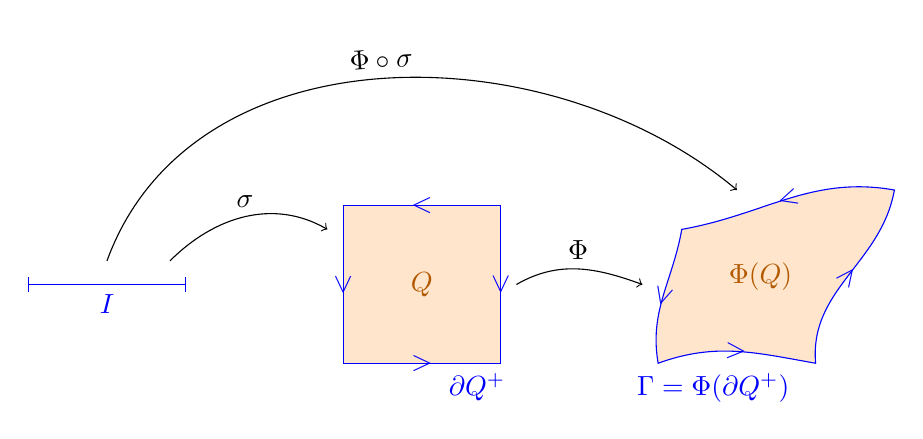
\begin{tikzpicture}
\draw[blue,|-|] (0,0) -- (2,0) node[midway,below] {$I$}; % Intervalo I

\draw[->] (1.8,0.3) to[out=45, in=150] node[midway,above] {$\sigma$} (3.8,0.7) ;

% % Primer cuadrado
\fill[orange!20!white,draw=none] (4,1) rectangle (6,-1);

\draw[blue] (4,-1) -- (4,1) node[midway,sloped] {\textless};
\draw[blue] (4,1) -- (6,1) node[midway,sloped] {\textless};
\draw[blue] (6,1) -- (6,-1) node[midway,sloped] {\textgreater};
\draw[blue] (6,-1) -- (4,-1) node[midway,sloped] {\textgreater};

\node[orange!70!black] at (5,0) {$Q$};
\node[blue,below] at (5.7,-1) {$\partial Q^+$}; 

\draw[blue, fill=orange!20!white] 
	(8,-1) to[out=100, in=260] node[midway,sloped] {\textless} 
	(8.3,0.7) to[out=10, in=170] node[midway,sloped] {\textless} 
	(11,1.2) to[out=260, in=95] node[midway,sloped] {\textgreater} 
	(10,-1) to[out=170, in=20] node[midway,sloped] {\textgreater}  (8,-1) -- cycle;

\draw[->] (6.2,0) to[out=30, in=160] node[midway,above] {$\Phi$} (7.8,0);	

\node[orange!70!black] at (9.3,0.1) {$\Phi(Q)$};
\node[blue,below] at (8.7,-1) {$\Gamma = \Phi(\partial Q^+)$};

\draw[->] (1,0.3) to[out=70, in=140] node[above,sloped] {$\Phi\circ\sigma$} (9,1.2);
\end{tikzpicture}
\caption{Esquema para la aplicación de Stokes en un cubo unidad}
\end{figure}

 Sea $\omega$ una k-forma en $\real^n$. Queremos calcular la integral de su diferencial en $Φ(Q)$.
 
\[
\int_{\Phi(Q)} \dif \omega = \int_Q \Phi^{\ast}\dif\omega = \int_Q \dif(\Phi^{\ast}\omega) = \int_{∂Q^{+}} \Phi^{\ast}\omega
\]

Donde $∂Q^{+}$ es la frontera del cubo $Q$ orientada debidamente. El último paso es aplicar el teorema anterior.

Sea $\appl{\sigma}{I}{∂Q}$. Entonces, $\appl{\Phi\circ\sigma}{I}{\Gamma}$, siendo $\Gamma$ la frontera de $\Phi(Q)$.

Aplicando esto a la integral que estamos calculando:

\[
\int_{\Phi(dQ^{+})} \omega \equiv \int{\Phi\circ\sigma(I)} = \int_I (\Phi\circ\sigma)^{\ast} \omega = \int_I \sigma^{\ast}\left(\Phi^{\ast}(\omega)\right) = \int_{\sigma(I)} \Phi^{\ast}\omega = \int_{∂Q}\Phi^{\ast}\omega
\]
Hemos llegado finalmente a que \[ \int_{∂Q^+} \Phi^{\ast} \omega = \int_{\Phi(∂Q^+)} \omega \]

Ahora querríamos dar el siguiente paso: 

\[\int_{\Phi(∂Q^+)} \omega = \int_{∂(\Phi^{\ast}(Q))} \omega \]

Es decir, que la imagen de la frontera sea la frontera de la imagen. Esto no es inmediato: en el cambio a coordenadas polares, por ejemplo, no se cumple a primera vista (ver figura \ref{imgCambioPolaresFrontera}). Cuando el ángulo (θ) se mantiene fijo y $r$ varía (segmentos azules), la imagen de esa parte de la frontera es un radio de la circunferencia, y cuando $r=0$ y variamos el ángulo (segmento verde) la imagen es un punto. 

\begin{figure}[hbtp]
\centering
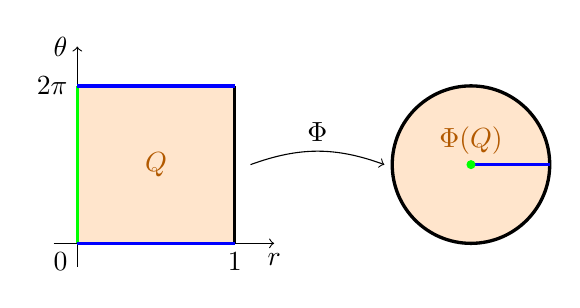
\begin{tikzpicture}
\fill[orange!20!white] (0,0) rectangle (2,2);

\draw[->] (0,-0.3) -- (0,2.5);
\node[left] at (0,2.5) {$\theta$};
\node[left] at (0,2) {$2\pi$};
\draw[->] (-0.3,0) -- (2.5,0);
\node[below] at (2.5,0) {$r$};
\node[below] at (2,0) {$1$};
\node[below left] at (0,0) {$0$};

\draw[very thick] (2,0) -- (2,2);
\draw[very thick,green] (0,0) -- (0,2);
\draw[very thick,blue] (0,2) -- (2,2);
\draw[very thick,blue] (0,0) -- (2,0);

\node[orange!70!black] at (1,1) {$Q$};

\draw[->] (2.2,1) to[out=20,in=160] node[midway,above,sloped] {$\Phi$} (3.9,1);

\draw[very thick,fill=orange!20!white] (5,1) circle (1);
\draw[very thick,blue] (5,1) -- (6,1);
\node[inner sep=1pt,circle,green,draw,fill=green] at (5,1) {};

\node[orange!70!black, above] at (5,1) {$\Phi(Q)$};

\end{tikzpicture}
\caption{La frontera no es la misma en el cambio a polares: las partes verde y azul forman parte de $∂Q$ pero no de $∂(Φ(Q))$.}
\label{imgCambioPolaresFrontera}
\end{figure}

Ahora bien, podemos dividir la región $Q$ en celdas disjuntas, como se puede ver en la figura \ref{imgPolaresDisjuntas}. De esta forma, las fronteras que sean comunes a varias celdas tendrán orientación incompatible y se anularán al integrar. Esto nos resuelve el problema y podemos enunciar el teorema de Stokes para celdas:


\begin{figure}[hbtp]
\centering
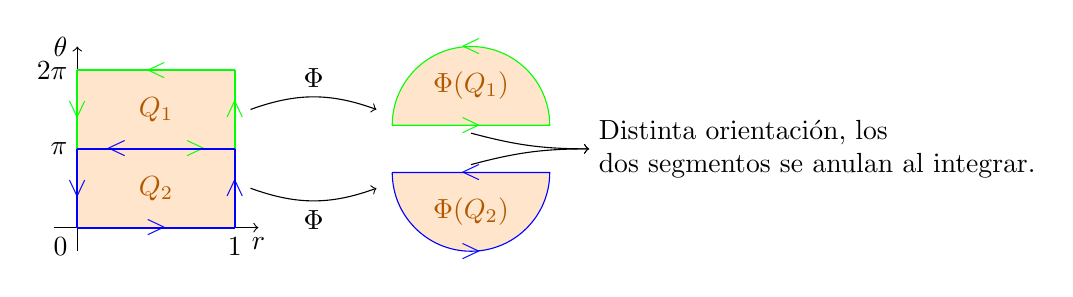
\begin{tikzpicture}
\fill[orange!20!white] (0,0) rectangle (2,2);

\draw[->] (0,-0.3) -- (0,2.3);
\node[left] at (0,2.3) {$\theta$};
\node[left] at (0,2) {$2\pi$};
\node[left] at (0,1) {$\pi$};
\draw[->] (-0.3,0) -- (2.3,0);
\node[below] at (2.3,0) {$r$};
\node[below] at (2,0) {$1$};
\node[below left] at (0,0) {$0$};

\draw[thick,green] (0,1) -- (0,2) node [midway,sloped] {\textless};
\draw[thick,green] (0,2) -- (2,2) node [midway,sloped] {\textless};
\draw[thick,green] (2,2) -- (2,1) node [midway,sloped] {\textless};
\draw[thick,green] (2,1) -- (0,1) node [near start,sloped] {\textgreater};

\draw[thick,blue] (0,0) -- (0,1) node [midway,sloped] {\textless};
\draw[thick,blue] (0,1) -- (2,1) node [near start,sloped] {\textless};
\draw[thick,blue] (2,1) -- (2,0) node [midway,sloped] {\textless};
\draw[thick,blue] (2,0) -- (0,0) node [midway,sloped] {\textgreater};

\node[orange!70!black] at (1,1.5) {$Q_1$};
\node[orange!70!black] at (1,0.5) {$Q_2$};

\draw[->] (2.2,1.5) to[out=20,in=160] node[midway,above,sloped] {$\Phi$} (3.8,1.5);
\draw[->] (2.2,0.5) to[out=-20,in=200] node[midway,below,sloped] {$\Phi$} (3.8,0.5);

\draw[green,fill=orange!20!white] (4,1.3) arc (180:0:1) -- (4,1.3) node[midway] {\textgreater};
\node[green] at (5,2.3) {\textless};
\node[orange!70!black] at (5,1.8) {$\Phi(Q_1)$};


\draw[blue,fill=orange!20!white] (4,0.7) arc (-180:0:1) -- (4,0.7) node[midway] {\textless};
\node[blue] at (5,-0.3) {\textgreater};
\node[orange!70!black] at (5,0.2) {$\Phi(Q_2)$};

\draw[->] (5,1.2) to[out=345, in=180] (6.5,1);
\draw[->] (5,0.8) to[out=15, in=180] (6.5,1);

\node[right,align=left] at (6.5,1) {Distinta orientaci\'{o}n, los\\ dos segmentos se anulan al integrar.};

\end{tikzpicture}
\caption{Podemos dividir $Q$ en dos celdas disjuntas}
\label{imgPolaresDisjuntas}
\end{figure}


\begin{theorem}[Teorema\IS de Stokes (para celdas)]\label{thmStokesCeldas}
\[ \int_M \dif \omega = \int_{\partial  M^+}\omega \]

, si la variedad $M$ se puede descomponer como unión de celdas con interior disjunto. 
\end{theorem} 

\paragraph{Frontera de una superficie}
Vamos a intentar definir en serio la frontera de objetos en $\real^3$, que es algo que necesitamos tener realmente muy claro.

\easyimg{imgs/StokesCeldasTipo.png}{ψ nos lleva $P$ a un punto que no está en la frontera de la imagen por ψ de su celda correspondiente (llamada de tipo I). En el caso de $Q$, ψ lo lleva a un punto en la frontera de la imagen de su celda por ψ (de tipo II), por lo tanto sí es un punto de la frontera.}{imgTiposCelda}

Hace un tiempo, cuando definíamos una subvariedad, demostramos la existencia de un difeomorfismo Ψ que "aplanaba un trozo" de subvariedad. La frontera de una superficie es el conjunto de los puntos (llamados en clase de Tipo 2) que al aplanar nos quedan en la frontera de un objeto de dimensión 2 (ver imagen \ref{imgTiposCelda}).
\index{Frontera}
Una vez aclarado el concepto de frontera, pasamos a demostrar el teorema de Stokes.


\begin{theorem}[Teorema\IS de Stokes]
Sea $M$ una subvariedad compacta, orientable, con frontera relativa $\partial  M$.

Entonces

\[\int_{\partial  M^+}\omega = \int_M \dif \omega \]

\end{theorem}

\begin{proof} La demostración ya está vista para celdas en la sección anterior, así que vamos a extender la idea.



\subparagraph{Paso 1: Compacidad}
Para todo punto $P\in M$ existe una celda $C_p$ tal que $P \in C_p$. Por lo tanto, está claro que $M\subset \bigcup_{p\in M} C_p$. Tomamos el interior de las celdas, para trabajar con conjuntos abiertos.

Hemos recubierto con infinitos abiertos la subvariedad, así que por compacidad (\ref{thmCerradoAcotado}) existe un subrecubrimiento \textbf{finito}.

Sin embargo, no podemos garantizar que las celdas son disjuntas. Si lo fueran, aplicaríamos el teorema a cada celda y listo. Hay que ver qué ocurre cuando las celdas no son disjuntas.

\subparagraph{Paso 2: Particiones de la unidad}

Vamos a intentar resolver el problema de los solapamientos. Buscamos una función que valga cero fuera de la celda que consideramos y sea mayor que cero dentro de ella, algo como pueda ser la figura \ref{imgStokesPhi}.

\begin{wrapfigure}{r}{0.6\textwidth}
  \begin{center}
    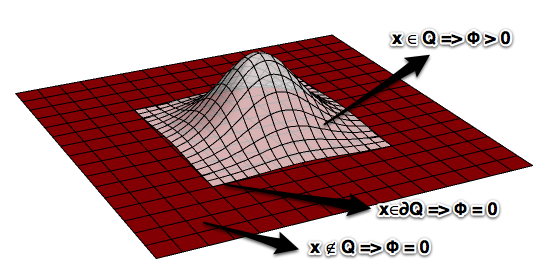
\includegraphics[width=0.58\textwidth]{imgs/TeoremaStokes-PartUnidad.png}
  \end{center}
  \caption{La función Φ que buscamos sería algo así.}
  \label{imgStokesPhi}
\end{wrapfigure}
Sea $\appl{\Phi}{\real^N}{\real}$. Además, 
\begin{itemize}
\item $\Phi>0$ en $\mathcal{Q}$
\item $\Phi = 0$ en $\partial  \mathcal{Q}$
\item $\Phi = 0$ en $\real^N-\mathcal{Q}$
\item $\Phi\in C^1$.
\end{itemize}
Consideramos $\Phi_i = \Phi\circ\Psi_{p_i}$, siendo $\Psi_{p_i}$ el difeomorfismo que cubre la celda $p_i$, con $i=1,...,k$ y la lleva al cubo unidad ($\mathcal{Q}$).

Además, nos gustaría que la suma de todas las aplicaciones $Φ_i$ sobre un punto sea 1:

\[ \sum_i \Phi_{i}(\gx) = 1\;\forall \gx \in M\]

Aunque parece una cosa imposible, vamos a ver que es algo perfectamente factible:

\[\tilde{\Phi}(\gx) = \frac{\Phi_i (\gx)}{\sum_{i=1}{k}\Phi_i(\gx)}\]

Estas $\tilde{\Phi}_i$ satisfacen todas las propiedades que nos interesan.

\subparagraph{Paso 3: Descomposición del problema}

Lo que nosotros queremos es calcular $\int_M d\omega$. Tal y como habíamos definido $\tilde{Φ}$ antes, es obvio que sobre la variedad $M$ 
\[ \omega=\sum_i^k\tilde{\Phi}_i(x)\omega \]

Entonces 

\[\dif \omega = \sum_{i=1}^k \dif (\tilde{\Phi}_i,\omega) = \sum_{i=1}^k \left( \dif \tilde{\Phi}_i\y \omega + \tilde{\Phi}_i \dif \omega \right) =  \dif\left(\sum_i \tilde{\Phi}_i\right) \y \omega + \sum \tilde{\Phi}_i \dif \omega\]

Dado que $\sum_i \tilde{Φ}_i = 1$, $\dif\left(\sum_i \tilde{\Phi}_i\right) = 0$ y por lo tanto

\[ \dif \omega = \sum \tilde{\Phi}_i \dif \omega \]

Aplicando esto descomponemos:
\[\int_M \dif \omega = \sum_{i=1}^k \int_M \tilde{\Phi}_i \dif\omega = \sum_{i=1}^k \int_{C_{p_i}} \tilde{\Phi}_i \dif\omega=\sum_{i=1}^k \int_{C_{p_i}} \dif(\tilde{\Phi}_i\omega)
\]

Hemos conseguido definir la integral como una suma finita de integrales sobre celdas en las que sí podemos aplicar el teorema de Stokes (\ref{thmStokesCeldas})

Entonces tenemos:

\[\int_M \dif \omega = \sum_{i=1}^k \int_{\partial  C_{P_i}^{+}} \tilde{\Phi}_i\omega\]

Por como hemos definido $\tilde{\Phi}_i$ tenemos que todas las celdas de tipo 1 valen 0. En cambio en las celdas de tipo 2 (ver \ref{imgTiposCelda} para los tipos de celda), tenemos una parte sobre la que $\tilde{\Phi}_i \neq 0$ (ver figura \ref{imgStokesCeldasIntegral}).

Esto nos deja: \[\int_M d\omega = \sum_{i=1}^k \int_{\partial  C{P_i}^{+}} \tilde{\Phi}_i\omega = \sum \int_{\partial M^+} \tilde{\Phi}_i \omega = \int_{\partial M^+} \omega\]

\end{proof}

\begin{figure}[hbtp]
  \begin{center}
    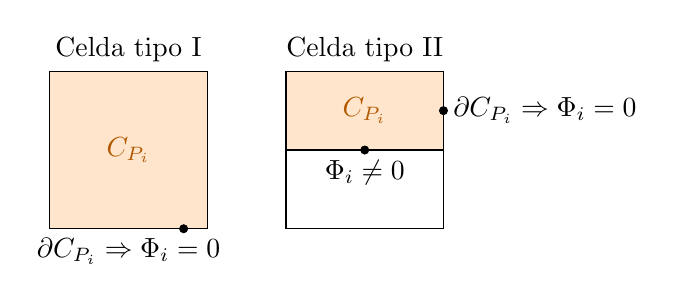
\begin{tikzpicture}
\draw[fill=orange!20!white] (0,0) rectangle (2,2);
\node[orange!70!black] at (1,1) {$C_{P_i}$};
\node[below] at (1,0) {$\partial C_{P_i} \Rightarrow \Phi_i = 0$};
\node[draw,circle,inner sep=1pt,black,fill=black] at (1.7,0) {};
\node[above] at (1,2) {Celda tipo I};

\draw[fill=white] (3,0) rectangle (5,2);
\draw[fill=orange!20!white] (3,1) rectangle (5,2);
\node[draw,circle,inner sep=1pt,black,fill=black] at (4,1) {};
\node[orange!70!black] at (4,1.5) {$C_{P_i}$};
\node[right] at (5,1.5) {$\partial C_{P_i} \Rightarrow \Phi_i = 0$};
\node[draw,circle,inner sep=1pt,black,fill=black] at (5,1.5) {};
\node[below] at (4,1) {$\Phi_i \neq 0$};
\node[above] at (4,2) {Celda tipo II};

\end{tikzpicture}
  \end{center}
  \caption{Sólo influyen a la integral los puntos de la frontera de la variedad, los que llevan a celdas de tipo II.}
  \label{imgStokesCeldasIntegral}
\end{figure}

\begin{example}
Sea $M$ una superficie en $\real^3$, un trozo de $x^2+y^2+z^2 = 1$ dentro de $x^2+y^2\leq y$, con $z\geq 0$. Ver figura \ref{imgEsferaCono}. Consideramos la orientación positiva como la de la normal hacia abajo.

\easyimg{imgs/EsferaCilindro.png}{Intersección de la esfera y el cilindro. La línea azul es la frontera de $M$, y las flechas naranjas indican su orientación positiva.}{imgEsferaCono}


Calcular las tres integrales

\[ \int_{\partial M} x \id y;\;\int_{\partial M} y \id z;\; \int_{\partial M} z \id x \]

\textbf{Previos} Nos damos cuenta de que $x^2+y^2\leq y$ es una circunferencia. Si completamos cuadrados tenemos la siguiente ecuación: \[x^2+\left(y-\frac{1}{2}\right)^2 = \frac{1}{4}\]

Es decir, una circunferencia de radio $\frac{1}{2}$ centrada en $(0,\frac{1}{2})$.

\paragraph{Resolución de $\int_{\partial M} x \dif y$}

\[
\int_{\partial M^{+}} x\dif y =\int_{\partial M^{+}} (0,x,0) \dif\sigma \stackrel{\mathrm{Stokes} }{=} \iint\limits_M \rot (0,x,0) \dif S = \iint\limits_M (0,0,1) \dif S
\]

Para calcular esta integral (que es calcular el flujo) aplicamos la fórmula de siempre. Para ello necesitamos parametrizar la superficie $M$:
\begin{equation}\label{eqEjStokes}
\Phi(x,y) = (x,y,\sqrt{1-x^2+y^2}), (x,y)\in D = \{x^2+y^2\leq y\} 
\end{equation}

Calculamos $T_x\x T_y =\displaystyle \left(\frac{x}{\sqrt{\cdot}},\frac{x}{\sqrt{\cdot}},1\right)$

\[
\int \int_M (0,0,1) dS = - \int \int_D \pesc{(0,0,1),(\ast,\ast,1)} \,dx\,dy = -\text{ Area } (D) = -\pi\frac{1}{4}
\]

\[ \int_{∂M^+}y\df{z} = \int_{∂M^+}(0,0,y)\df{σ} \stackrel{Stokes}{=} \int\int_{M^+} \rot (0,0,y)\df{S} \]

En \ref{eqEjStokes} teníamos la parametrización, así que la aplicamos. Teniendo en cuenta la orientación, tenemos que cambiar el signo y nos queda 

\[ 
- \iint_D \pesc{(1,0,0),\left(\frac{x}{\sqrt{\ast}}, \frac{y}{\sqrt{\ast}}, 1}\right) \df{x}\df{y} 
= -\iint_D\frac{x}{\sqrt{1-x^2-y^2}} \d{x,y} 
\]

Viendo que estamos integrando una función impar en una región simétrica, la integral vale 0.

\paragraph{Resolución de $\int_{\partial M} z \dif x$}

Pasamos ahora a calcular la integral de $z$. Tenemos lo mismo que antes:

\begin{gather*}
 \int_{∂M^+}z\df{x} = \int_{∂M^+}(z,0,0)\df{σ} \stackrel{Stokes}{=} \iint_{M^+} \rot (z,0,0)\df{S} = \iint_{M^+}(0,1,0)\id{S}= \\
 - \iint_D \pesc{(0,1,0),\left(\frac{x}{\sqrt{\ast}}, \frac{y}{\sqrt{\ast}}, 1\right)}\id{x,y} 
= -\iint_D\frac{y}{\sqrt{1-x^2-y^2}} \id{x,y}
\end{gather*}

Vemos que esta integral es muy complicada y nos va a ganar, así que pasamos a tratar de integrar como una curva. Deberemos parametrizar la curva, encontrar la orientación correcta y aplicar la fórmula.

Empezamos con la parametrización:

\[ ∂M = \left\{ \begin{matrix}
x^2+y^2+z^2 = 1 \implies y + z^2 = 1 \implies z = \sqrt{1-y} \\
x^2 + y^2 = y \implies x = \pm \sqrt{y-y^2}
\end{matrix}\right. \]

Por lo tanto, podemos parametrizar en dos trozos

\begin{align*}
Γ_1\equiv &(\sqrt{y-y^2}, y, \sqrt{1-y});\;y∈[0,1] \\
Γ_2\equiv &(-\sqrt{y-y^2}, y, \sqrt{1-y});\;y∈[0,1] \\
\end{align*}

\easyimgw{imgs/OrientacionesEsferaCilindro.png}{Orientaciones de $Γ_1$ y $Γ_2$}{imgOrientacionesEsferaCilindro}{0.7}

Tal y como vemos en la figura \ref{imgOrientacionesEsferaCilindro}, la orientación es negativa en $Γ_1$ y positiva en $Γ_2$. Entonces

\[ \int_{∂M^+}(z,0,0)\df{σ} = \int_{Γ_1^+}(z,0,0)\dif{σ_1} +  \int_{Γ_2^+}(z,0,0)\dif{σ_2} \]

Operando con la primera integral:

\[  \int_{Γ_1^+}(z,0,0)\dif{σ_1} = - \int_0^1\pesc{(\sqrt{1-y},0,0),\left(\frac{1-2y}{2\sqrt{y-y^2}},\ast,\ast\right)}\dif y = 
-\int_0^1\frac{1-2y}{2\sqrt{y}}\dif y = \]

Separamos en dos sumandos

\[ = \int_0^1\sqrt{y}\d y - \int_0^1 \frac{1}{2\sqrt y}\dif y = \dotsb \]

Podríamos tomar otra parametrización alternativa usando coordenadas esféricas. La esfera queda determinada por la parametrización

\[ \left\{\begin{matrix}
x &=& \cos θ \sin φ \\
y &=& \sin θ \sin φ \\ 
z &=& \cos φ
\end{matrix}\right. \]

Añadiendo la restricción de $x^2+y^2=y$, nos queda que $\sin φ = \sin θ$. Entonces podemos seguir parametrizando 

\[\left. \begin{matrix}
x = \cos θ \sin θ \\
y = \sin^2 θ \\
 z = \sqrt{1-\sin^2 θ} = \abs{\cos θ}
\end{matrix} \right\} θ∈[0,π]
\]

y tenemos que

\[ σ_1(θ) = (\cos θ \sin θ, \sin^2 θ, \cos θ) \]

Por otra parte, si pusiésemos los límites de integración en la región D pasaría algo.
\end{example}

\section{Campos conservativos}

\begin{defn}[Campo\IS conservativo] Consideramos $\vf$, un campo en $ℝ^N$. Se dice que $\vf$ es conservativo si y sólo si $∃\appl{V}{ℝ^N}{ℝ}$ tal que $F=\grad V$, donde $V$ es el \textbf{potencial}\index{Potencial} del campo $\vf$.
\end{defn}

\begin{theorem} Sea $\vf$ un campo $C^1$ en $ℝ^3$. Entonces $\vf $ es conservativo si y sólo si $\rot \vf = \vec{0}$.
\end{theorem} \label{consImpRot}

\begin{proof}
\paragraph{Implicación a la derecha} Como $F=\grad V$, y $F∈C^1$, entonces $V∈C^2$. Calculamos ahora el rotacional:

\[ \rot\vf = \left|\begin{matrix}
\vec{i} & \vec{j} & \vec{k} \\
\pd{}{x} & \pd{}{y} & \pd{}{z} \\
F_1 & F_2 & F_3
\end{matrix}\right| = \left(\dpa{F_3}{y}-\dpa{F_2}{z}, \dpa{F_1}{z}-\dpa{F_3}{x}, \dpa{F_2}{x}-\dpa{F_1}{y} \right) \]

Sustituyendo con $F=\grad V$ veríamos que sale todo cero.

\paragraph{Implicación hacia la izquierda}

Supongamos $Γ$ una curva cerrada, que sea la frontera de una superficie $M$. Entonces

\[ \int_{M^+}\vf  \stackrel{Stokes}{=} \iint_M\rot \vf\dif S = 0 \]

Es decir, que la integral de $F$ sobre cualquier curva cerrada va a dar 0. Buscamos ahora un $V$ tal que $\grad V = \vf$.

Supongamos un punto cualquiera $(x,y,z)$: A ese punto podemos llegar a través de varias rectas paralelas a los ejes. Con esas rectas podríamos construir un camino, y entonces tendríamos que 

\todo[inline]{Poner dibujito aquí}

\[ \int_{Γ_1}\vf = \int_{Γ_2} \vf = \int_{Γ_3}\vf \]

ya que cogiendo dos pares $Γ_i$ y cambiando la orientación de uno de ellos construimos una curva cerrada.

Parametrizamos $Γ_1$:

\[ Γ_1 \equiv \{ (t,0,0)\,t∈[0,x]\} 
	\cup \{ (x,s,0)\,s∈[0,y]\}
	\cup \{ (x,y,r)\,r∈[0,z]\} \]
	
Entonces

\begin{align*}
\int_{Γ_1}\vf&= \int_0^x\pesc{(F_1(t,0,0),F_2(t,0,0), F_3(t,0,0),(1,0,0)}\dif t \\
&+\int_0^y\pesc{(F_1(x,s,0),F_2(x,s,0), F_3(x,s,0),(0,1,0)}\dif s \\
&+\int_0^x\pesc{(F_1(x,y,r),F_2(x,y,r), F_3(x,y,r),(1,0,0)}\dif r \\
&=\int_0^x F_1(t,0,0)\dif t + \int_0^y F_2(x,s,0)\dif s+ \int_0^z F_3(x,y,r)\dif r 
\end{align*}

De la misma forma, tendríamos

\begin{gather*}
\int_{Γ_2}\vf = \int_0^y F_2(0,t,0)\dif t + \int_0^z F_3(0,y,s)\dif s+ \int_0^x F_1(x,y,r)\dif r \\ 
\int_{Γ_3}\vf = \int_0^x F_1(t,0,0)\dif t + \int_0^z F_3(x,0,s)\dif s+ \int_0^y F_1(x,r,z)\dif r \\
\end{gather*}

Las tres integrales son iguales, así que podemos derivar con respecto de la que nos venga mejor para construir la función $V$, que es la que buscábamos.

\end{proof}

La versión de este teorema vista en clase de prácticas (que es una versión más práctica)
\begin{theorem}[Campos conservativos]
$F$ es un campo vectorial $C^1$ en $\real^3$ excepto en un número finito de puntos entonces son equivalentes:
\begin{itemize}
\item Existe un potencial
\item La integral sobre una curva cerrada simple es 0
\item Las integrales por un camino o por otro para llegar a un punto son iguales
\item rot $\vf=0$.
\end{itemize}
\end{theorem}

Además, para calcular el potencial se puede utilizar cualquiera de estas 3 fórmulas:

\begin{gather*}
\int_{Γ_1}\vf=\int_0^x F_1(t,0,0)\dif t + \int_0^y F_2(x,s,0)\dif s+ \int_0^z F_3(x,y,r)\dif r \\
\int_{Γ_2}\vf = \int_0^y F_2(0,t,0)\dif t + \int_0^z F_3(0,y,s)\dif s+ \int_0^x F_1(x,y,r)\dif r \\ 
\int_{Γ_3}\vf = \int_0^x F_1(t,0,0)\dif t + \int_0^z F_3(x,0,s)\dif s+ \int_0^y F_1(x,r,z)\dif r \\
\end{gather*}

\subsection{Ejemplos}

\begin{example} Tenemos un cono de base $D$ y altura $h$, y buscamos integrar el campo $\vf(x,y,z)= (x,y,z)$. $Ω$ es el espacio del cono, y $∂Ω$, su superficie, se divide en la superficie lateral y la base.

\todo[inline]{Dibujito L1244}

Si escribimos el teorema de Gauss, tenemos que 

\[ \iiint_Ω \dv \vf \id{x,y,z} = \iint_{∂Ω^+} \vf \dif S \]

En este caso, tenemos la suerte de que $\dv \vf = 3$, y por lo tanto

\[ \iiint_Ω \dv \vf \id{x,y,z} = 3 \cdot \mathrm{Volumen}\,(Ω) \]

Por lo tanto, para hallar el volumen calculamos la integral sobre la superficie y dividimos entre tres.

La idea geométrica es que en la cara lateral, la componente normal de $\vf$ es 0. Lo vemos fácilmente sabiendo que la recta definida por el vector $(x,y,z)$ y que pasa por el origen (el vértice del cono), tiene exactamente la misma dirección de la generatriz. Entones,\textbf{ la integral sobre la cara lateral es 0} y por lo tanto podemos ignorarla. Nos centramos sólo en la integral de la base:

\[ \iint_{\mathrm{Base}}\vf \id S \]

Parametrizar $S$ es sencillo:

\[ S \equiv \{ (x,y,h)\tq (x,y)∈ D \} \]

Calculamos su vector normal:

\[ \left.\begin{matrix}
T_x = (1,0,0) \\
T_y = (0,1,0)
\end{matrix}\right\} T_x × T_y = (0,0,1) \]

y entonces

\[ \iint_{\mathrm{Base}}\vf \id S = \iint_D\pesc{(x,y,h),(0,0,1)} \id{x,y} = \iint_D h \id{x,y} = h \cdot \mathrm{Area}\,(D) \] 

Finalmente 

\[ \mathrm{Volumen}\,(Ω) = \frac{h \cdot \mathrm{Area}\,(D)}{3} \]
\end{example}

\begin{example}[Cálculo del campo eléctrico o gravitatorio]

La expresión del campo eléctrico es 

\[ \vf(\vx) = C \frac{\vx}{\norm{\vx}^3} \]

Calculando las derivadas parciales

\begin{align*}
\dpa{F_1}{x}&=\frac{y^2+z^2-2x^2}{(x^2+y^2+z^2)^{\frac{5}{2}}} \\
\dpa{F_2}{y}&=\frac{x^2+z^2-2y^2}{(x^2+y^2+z^2)^{\frac{5}{2}}} \\
\dpa{F_3}{z}&=\frac{x^2+y^2-2z^2}{(x^2+y^2+z^2)^{\frac{5}{2}}}
\end{align*}

nos queda que

\[ \dv\vf = 0 \]

Consideramos ahora una bola de radio $R$ centrada en el origen, es decir, $B_R(0,0,0)$. Integramos sobre su superficie:

\[ \iint\limits_{∂B_R^+} \vf \id{S} = 
\iint\limits_{B_R} \left(\frac{x}{R^3},\frac{y}{R^3},\frac{z}{R^3} \right) \id S = \frac{1}{R^3} \iint\limits_{B_R} (x,y,z)\id S = \]

Dado que integrar el vector es integrar su componente escalar, la integral nos queda

\[ = \frac{1}{R^3} \iint\limits_{B_R} R\id{x,y} = \frac{1}{R^2}\cdot \mathrm{Area\; esfera} = 4π \]

Ahora bien, si no supiésemos ese argumento geométrico, empezaríamos parametrizando la esfera:

\[ Φ(θ,φ) =(R\cos θ \sin φ, R\sin θ\sin φ, R\cos φ);\, θ∈[0,2π], φ∈[0,π] \]

Calculamos los vectores tangentes y el normal:

\[ \begin{matrix} \\ T_θ = \\ T_φ= \end{matrix}
\left|
\begin{matrix}
\vec{i} 		& \vec{j} 		 & \vec{k} \\
-R\sin θ \sin φ & R\cos θ \sin φ & 0 \\
R\cos θ\cos φ 	& R\sin θ \cos φ & -R\sin φ
\end{matrix}\right|: T_θ×T_φ = -R\sin (R\cos θ, \]

La normal es interior, así que pagamos con un cambio de signo:

\begin{gather*} \iint\limits_{x^2+y^2+z^2 = R^2} \left(\frac{x}{R^3},\frac{y}{R^3},\frac{z}{R^3} \right) \id S = \\
- \int_0^{2π}\int_0^π\pesc{\left(\frac{R\cos θ \sin φ}{R^3},{R\sin θ \sin φ}{R^3},{R\cos φ}{R^3}\right), (,,)} = \dotsb \mathrm{Calculos\; aqui} \end{gather*}

y al final sale lo mismo que antes pero con cuentas mucho más desagrable.

¿Por qué el teorema de Gauss no funciona? La divergencia es 0 y la superficie es cerrada. Sin embargo, $\vf$ no es $C^1$ en el origen (no existe en ese punto) así que no podemos aplicarlo.

Pero, por otra parte, siempre hemos visto que la integral no se ve afectada por lo que ocurra en un punto. ¿Por qué no funciona el teorema de Gauss sólo por lo que pasa en el origen?

En realidad en el origen la divergencia vale $4π$ por la Delta de Dirac (δ).

Pero también podemos hacer un apaño. Consideramos un conjunto $Ω$, y una bola $B_ε(0,0,0)$. Entonces

\[ Ω_ε = Ω - B_ε \]

de tal forma que $\vf∈C^1$ en $Ω_ε$. Aplicando el teorema de Gauss:

\[ 0 = \iiint\limits_{Ω_ε}\dv \vf \id{x,y,z} = \iint\limits_{∂Ω_ε^+}\vf \id{S} \]

La frontera se divide en dos partes: $∂Ω_ε = ∂Ω + ∂B_ε^+$. Entonces

\[ 0 = \iint\limits_{∂Ω^+}\vf \id S - \iint\limits_{∂B_ε^+}\vf \id S \]

y por lo tanto, tenemos que 

\[ \iint\limits_{∂Ω^+}\vf \id{S} = 4π\; ∀Ω \tq 0 ∈ Ω \]

\end{example}


\begin{theorem} Dado un campo $\vf \in C^1$, se tiene que
\[ \dv \vf = 0\dimplies \exists \vg\in C^2 \tlq \rot \vg = \vf \]
\end{theorem}

\begin{proof}

Con el lenguaje de las formas diferenciales es muy fácil esta demostración.

\todo[inline]{reescribir bien}
$\vf$ es una 1-forma a la que aplicamos la diferencial exterior y obtenemos una 2-forma, que es su rotacional. Entonces, al volver a hacer la diferencial (para hallar la divergencia) estamos aplicando dos veces el diferencial, y por lo tanto su valor es 0.

Sin formas diferenciales tenemos:

\[G=(G_1,G_2,G_3)\]
\[\rot G = \left(\ast_1,\ast_2,\ast_3\right)\]

\[\dv(\rot G) = \dpa{}{x}(\ast_1) + \dpa{}{y}(\ast_2) + \dpa{}{z}(\ast_3)\]
Por la igualdad de las derivadas cruzadas (toerema de Euler) al ser $G\in C^2$ se cancela todo.

$\implies$ Buscamos $\vg$ tal que $(F_1,F_2,F_3) = \rot \vg$.

Podemos definir el sistema:

\[\begin{array}{cc}
\dpa{G_3}{y} - \dpa{G_2}{z} &= F_1\\
\dpa{G_1}{z} - \dpa{G_3}{x} &= F_2\\
\dpa{G_2}{x} - \dpa{G_1}{y} &= F_3
\end{array}\]

Como tenemos varios grados de libertad, supongamos que $G_3\equiv 0$

\[\begin{array}{cc}
 - \dpa{G_2}{z} &= F_1\\
\dpa{G_1}{z} - &= F_2\\
\dpa{G_2}{x} - \dpa{G_1}{y} &= F_3
\end{array} \begin{array}{cc}
\longrightarrow & G_2 = -\int_0^z F_1(x,y,t)dt+A(x,y)\\
\longrightarrow & G_1 = \int_0^2 F_2(x,y,t)dt + B(x,y)\\
\longrightarrow & F_3 = \dpa{}{x} \left\{-\int_0^z F_1(x,y,t)dt + A(x,y)\right\}
- \dpa{}{y}\left\{\int_0^2 F_2(x,y,t)dt + B(x,y) \right\}
\end{array}
\]

Vamos a ver que ocurre con  $F_3$

\[-\dpa{}{x}\left(\int_0^z F_1(x,y,t)dt\right) + \dpa{A}{x} - \dpa{}{y}\int_0^z F_2(x,y,t)dt - \dpa{B}{y}\]

Por la regularidad de $F_1$ podemos meter dentro la derivada (el argumento que está detrás de esto se ve en teoría de la medida, asíque de momento nos fiamos)

\[-\left(\int_0^z \dpa{}{x}F_1(x,y,t)dt\right) + \dpa{A}{x} - \int_0^z \dpa{}{y}F_2(x,y,t)dt - \dpa{B}{y}\]
\[-\int_0^z \left(\dpa{F_1}{x} + \dpa{F_2}{y}\right)(x,y,t)dt + \dpa{A}{x} - \dpa{B}{y} \]

Utilizamos que la $\dv = 0$ que nos dice:

\[\dpa{F_1}{x} + \dpa{F_2}{y} + \dpa{F_3}{z} = 0\]

\[ = \int_0^z \dpa{F_3}{z} (x,y,t)dt + \dpa{A}{x} - \dpa{B}{y} = F_3(x,y,z) - F(x,y,z) + \dpa{A}{x} - \dpa{B}{y}\]

Hemos llegado a \[F_3(x,y,z) =  F_3(x,y,z) - F(x,y,z) + \dpa{A}{x} - \dpa{B}{y}\]
Quedando entonces definidas $A$ y $B$ así:

\[\dpa{A}{x} - \dpa{B}{y} = F_3(x,y,0)\]
Y aquí nuevamente tenemos muchas opciones. Tomamos $B=0$ por tomar algo

\[A(x,y) = \int_0^x F_3(s,y,0)ds + C(y)\]
\end{proof}

\subsubsection{Anexo interesante}
Vamos a ver ahora un ejemplo de cuándo se pueden meter las derivadas dentro de una integral.

\begin{example}
Tenemos un sólido a una cierta temperatura, rodeado de un amniente a otra temperatura distitnta de tal manera que el sólido va perdiendo temperatura. Queremos saber a qué temperatura estará el sólido pasa un tiempo $T$.

Partimos de la interpretación de que la temperatura mide la \emph{cantidad de calor}. 

\textbf{Concepto previo} Una olla de 100 Litros y un vasito de chupito, ambos con agua a 100 grados, ¿qué recipiente tiene más energía? Respuesta: la olla porque es más grande.

\todo{creo que es así}
Podemos calcular el calor integrando la temperatura con el volumen


Siendo $\Omega$ el sólido, y $u(x,t)$ es la temperatura en $x$ en el instante $t$. Entonces:

\[\iiint u(x,t) dx \equiv \text{ Cantidad de calor en }\Omega\text{ en }t\]

Vamos a tomar una $B_{\epsilon}(x_0)$, vamos a estudiar:
\[\dpa{}{t} \iiint_{B_{\epsilon}(x_0)} u(x,t)dx\]
 Es la variación de temperatura a lo largo del tiempo. La temperatura varía porque el calor se transmite. ¿De qué manera se transmite? Sale fuera a través de la frontera. Se habrá ganado el calor que haya entrado y se habrá perdido el calor que haya salido. ¡Es un flujo!
 (de un campo $\vec{J}$)
  
 \[\dpa{}{t} \iiint_{B_{\epsilon}(x_0)} u(x,t)dx = -\iint_{\partial B_{\epsilon}(x_0)} \vec{J}dS\]
 (El menos aparece porque queremos que la derivada sea negativa, porque el calor sale.)
 
 
 Siguiendo la idea de Leibniz de que estamos en el mejor mundo posible ,porque el calor se transmite de las zonas calientes a las zonas frías de la manera óptima, es decir, en la dirección del $-\grad$.
 
 \todo[inline]{Revisar que pasa con $\dpa{}{t}$}
 
 \[\dpa{}{t} \iiint_{B_{\epsilon}(x_0)} u(x,t)dx = -\iint_{\partial B_{\epsilon}(x_0)} \vec{J}dS = \iint_{\partial B_{\epsilon}(x_0)}\]
 \[ = -\grad_x u dS \stackrel{Gauss}{=} \iiint_{B_{\epsilon}(x_0)} \dv(\grad_x u) = \iiint_{B_{\epsilon}(x_0)}  \]

\[ = \iiint_{B_{\epsilon}(x_0)} \dpa{u}{t}-Au\,dx=0,\forall \epsilon\]

Como lo que integramos es continua (lo llamamos $f$)

Tenemos:
\[m_{\epsilon} \leq \frac{1}{Vol(B_{\epsilon})} \iiint f \leq M_{\epsilon}\] 

Si $\epsilon \to 0$ entonces $\displaystyle\iiint_{B_{\epsilon}(x_0)} f = f(x_0)$

Entonces tenemos que \[\dpa{u}{t}(x_0,t) - Au(x_0,t) = 0\]

Y de aquí deducimos las 3 ecuaciones de transmisión de calor, que son: 
\todo[inline]{no se cuales son}
 \end{example}

Para este ejemplo ha sido fundamental el meter dentro una derivada ($\dpa{}{t}$) dentro de la integral.

Ahora vamos a ver otro ejemplo en el que esto no se puede aplicar:

\begin{example}
\todo{Dibujo}
\[\int_0^1 f_n(x)dx = \frac{1}{2}\]
\[\lim_{n\to\infty}\int_0^1 f_n(x)dx = \frac{1}{2}\]
\[\int_0^1 \lim_{n\to\infty} f_n(x) = \int_0^1 0dx = 0\]

Estamos cometiendo un error... que no vamos a contar cuál es, que se verá en teoría de la medida.
\end{example}

Nos podemos plantear en qué condiciones es cierto (en el ejemplo anterior es falso):

\[\lim_{n\to\infty} \int_{\Omega}\frac{u(x,t+1/u)-u(x,t)}{1/u} \,dx = \int_{\Omega}\lim_{n\to\infty}\frac{u(x,t+1/u)-u(x,t)}{1/u} \,dx
\]

Lo primero que tenemos que definir es la \textbf{convergencia de una sucesión a una función.} Vamos a ver un plan de interpretaciones.

\subparagraph{\textit{Convergencia puntual}}

$\forall x\in\Omega$, dado un $\epsilon>0\\ \exists n_0 \tlq n>n_0 \implies \abs{f_n(x)-f(x)}<\epsilon$

\begin{example}
1) \[f(x) = \left\{\begin{array}{cc}
1 & x\in[0,1]\cap \rac\\
0 & x\in[0,1]\cap\{\real-\rac\}
\end{array}\right.\]
Este es el ejemplo de función no integrable por Riemman (las sumas superriores valen 1 y las sumas inferiores valen 0, debido a la numerabilidad de los Racionales)

2)
Nosotros podemos definir una función de la siguiente manera: 

\[f_n(x) = \left\{\begin{array}{cc}
1 & x=r_1,...,r_n\\
0 & x\in\real-\{r_1,...,r_n\}
\end{array}\right\}\]
Siendo $r_i\in\rac$. Como es un conjunto numerable podemos definir un orden.

Continua excepto en un nº finito de puntos $\implies$ integrable de Riemman.

3) $f_n(x)\to f(x) \forall x\in[0,1]$


\textbf{Conclusión} En este caso tenemos que la convergencia puntual podemos no tener integral. 
\end{example}

Para solucionar este problema podemos definir otra noción de límite que nos evite este problema u otra noción de integral.

\subparagraph{\textit{Convergencia uniforme}}

Dado $\epsilon>0\,\exists\,n_0=n_0(\epsilon) \tlq n_0>n_0 \implies \abs{f_n(x) - f(x)} < \epsilon\, \forall x\in\Omega$.

Es decir, ${sup}{x\in\Omega} \abs{f_n(x)-f(x)} = \md{f_n-f}_{\infty} <\epsilon$.

La misma idea que con continuidad uniforme, para todos los $x$ del intervalo nos vale el mismo $n_0$.

Utilizando esta definición en el ejemplo de los triángulos, no podemos definir la sucesión que sea convergente uniformemente.

\begin{theorem}[Convergencia uniforme]
Sea $\Omega$ un dominio acotado en $\real^N$. 

Si $f_n \to f$ converge uniformemente en $\Omega$

\textbf{entonces}
\[\lim_{n\to\infty} \int_{\Omega} f_n(x)\,dx = \int_{\Omega} \lim_{n\to\infty} f_n(x)\,dx = \int_{\Omega} f(x)\,dx\]

Es decir, el límite y la integral son intercambiables.
\end{theorem}

\begin{proof}
\[0\leq\abs{\int_{\Omega}f_n(x) - f(x) \, dx} \leq <\int_{\Omega} \epsilon \,dx =\epsilon\abs{\Omega} \to 0\]
\end{proof}

\begin{theorem}
\[\left.\begin{array}{cc}
\{f_n\} \text{ continua }\\
f_n \to f \text{ uniforme en } \Omega \end{array}
\right\} \implies f \text{ continua}\]
\end{theorem}
\obs Si tenemos convergencia unifirme, tenemos una función continua. Parace una cosa tan tan buena que incluso se pasa de buena, porque no podemos trabajar con discontinuidades

\obs Adelantamos un teorema de teoría de la medida que dice \textit{ Casi todas las funciones son casi continuas en casi todos los puntos}


\begin{proof}
\[\abs{f(x) - f(y)} = \abs{f(x) \pm f_n(x) \pm f_n(y) - f(y)}\]

Elegimos un subíndice $n$ para el que se cumpla $\abs{f_n(t) - f(t)} < \frac{\epsilon}{3}$

Además, como $f_n$ son continuas, tenemos que haciendo tender $x\to y \implies f(x) - f(y) \leq \epsilon \implies$ continuidad
\end{proof}


\paragraph{Aplicación}

Sea $f_n(x) = \frac{u(x,t+1/u) - u(x,t_0)}{1/u}$

$f(x) = \dpa{u}{u}(x,t_0)$

Vamos a comprobar la convergencia uniforme:

\[0\leq \abs{f_n(x) - f(x)} \leq \abs{\frac{u(x,t+1/u) - u(x,t_0)}{1/u} - \dpa{u}{u}(x,t_0)} \stackrel{TVM}{=} \abs{\dpa{u}{t}(x,s) - \dpa{u}{t}(x,t_0)} < \epsilon \forall x\]
Donde $s\in [t_0,t_0+\frac{1}{n}]$

En el último paso utilizamos la continudad de la derivada y la compacidad (que nos da continuidad uniforme)


\subparagraph{Integral de Lebesgue}
La otra opción para poder intercambiar límites con integrales podíamos ser más estrictos con la convergencia, o mejorar la integral (aparte de todo un mundo de posibilidades intermedias del \textit{Análisis funcional}) 

Algo de esto ya vimos al hablar de integrales: (\ref{IntLebesgue})

Esto nos genera el problema de la medida de un intervalo. 
Es razonable pedir:
\begin{itemize}
\item $\abs{(a,b)} = \abs{b-a}$
\item La medida del intervalo tiene que ser invariante si le aplicamos traslaciones
\item $A\cap B = Ø $

$\abs{A \cup B} = \abs{A} + \abs{B}$
\item $A_i \cap A_j = Ø, i\neq j$

$\abs{\bigcup_{i=1}^{\infty} A_i} = \sum_{i=1}^{\infty} \abs{A_i}$.


\end{itemize}
El último requisito es un verdadero dolor de cabeza, trabajar con sumas infinitas y con uniones infinitas. Sería fácil (con la medida exterior) para conseguir un $\leq$ que no es suficiente.

Para solucionar todo estos problemas hay que definir una nueva teoría con la que casi todo es medible (salvo unos cuantos monstruos, que para encontrarlos hay que hablar del Axioma de elección)

Toda esta teoría de la integral de Lebesgue nos da resultados mucho más generales para poder intercambiar el límite con la integral, con la convergencia monótona y la convergencia domiante.
